
\documentclass[AMA,LATO1COL]{WileyNJD-v2}
%demo
\usepackage{comment}
\usepackage{amssymb}
\usepackage{tikz}
\articletype{Article Type}%

\newcommand\bigo{\mathcal O}
\newcommand{\gpu}{\textsc{GPU}}
\newcommand{\gpus}{\textsc{GPU}s}
\newcommand{\cpu}{\textsc{CPU}}
\newcommand{\cpus}{\textsc{CPU}s}
\newcommand{\cuda}{\textsc{Cuda}}
\newcommand{\oneexp}{1\textbf{EXP}}

\raggedbottom

\begin{document}

\title{Fast LRT Implementation \\on Parallel Computer Architectures}

\author[1]{Author One*}

\author[2,3]{Author Two}

\author[3]{Author Three}

\authormark{AUTHOR ONE \textsc{et al}}


\address[1]{\orgdiv{Org Division}, \orgname{Org Name}, \orgaddress{\state{State name}, \country{Country name}}}

\address[2]{\orgdiv{Org Division}, \orgname{Org Name}, \orgaddress{\state{State name}, \country{Country name}}}

\address[3]{\orgdiv{Org Division}, \orgname{Org Name}, \orgaddress{\state{State name}, \country{Country name}}}

\corres{*Corresponding author name, This is sample corresponding address. \email{authorone@gmail.com}}

\presentaddress{This is sample for present address text this is sample for present address text}

\abstract[Summary]{The Likelihood Ratio Test (LRT) is a method for identifying hotspots or anomalous rectangular regions for an spatial data grid that draws from an arbitrary distribution.  LRT has wide-spread applications from social-media applications powered by mobile phones to medical image processing applications. Unfortunately, a na\"ive implementation of LRT exhibits a worst-case time complexity of $\bigo(n^4)$ for a two-dimensional grid.

For larger grids with a grid size of more than $64\times 64$ cells, a na\"ive implementation of LRT becomes intractable~\cite{jour} and it takes around several days to execute Grid(64,64) on a single-core CPU.

In this paper, we propose a parallel processing scheme for LRT computations for one parameter exponential (1EXP) distribution for multi-dimensional spatial data grids. The parallel processing scheme transforms LRT computations to a balanced embarrassingly parallel problem utilising a novel range mapping scheme. The new range mapping scheme relies on a dynamic pre-computation algorithm, and exhibits a worst-case complexity of $\bigo(n^2)$  for two dimensional spatial data-grids improving the complexity class by an order of two. Experiments were conducted for various computer architectures and platforms including shared-memory multi-core machines, multi-GPGPU computers, and the EC2 cloud computer. Extensive experiments are provided to demonstrate the utility of this approach and extensive performance analysis is given.
In the experiments we could achieve speedups up to $20,000$ times using our parallel processing scheme on Grid $(1000,1000)$.
}

\keywords{Spatial outlier, Likelihood Ratio Test, one parameter exponential distribution, Inclusive/Exclusive Principle, GPGPUs, Multi-core, EC2 Cloud Cluster}

\jnlcitation{\cname{%
\author{Williams K.},
\author{B. Hoskins},
\author{R. Lee},
\author{G. Masato}, and
\author{T. Woollings}} (\cyear{2016}),
\ctitle{A regime analysis of Atlantic winter jet variability applied to evaluate HadGEM3-GC2}, \cjournal{Q.J.R. Meteorol. Soc.}, \cvol{2017;00:1--6}.}

\maketitle

\section{Introduction}\label{sec1}
With the widespread availability of GPS-equipped smartphones and mobile
sensors, there has been an urgent need to perform large scale spatial data analysis.
For example, by carrying out a geographic projection of Twitter feeds, researchers are able to
narrow down ``hotspot'' regions where a particular type of activity is attracting a disproportionate  amount of attention. In neuroscience, high resolution MRIs facilitate the precise detection and localisation of regions of the brain which may indicate mental disorder.
The statistical method of choice for identifying hotspots or anomalous regions
is the Likelihood Ratio Test (LRT) statistic.
Informally, the LRT of a spatial region compares the likelihood of the given spatial region with its complement, and hence can be used to identify hotspot regions. In \cite{chisquare}, it was shown that the LRT value follows a $\chi^{2}$ distribution, independent of the distribution of the underlying data.

\noindent For a $n\times n$ spatial grid, the worst-case execution time for identifying the most
anomalous region is $\bigo(n^4)$. The reason for this high complexity class is that we have $\bigo(n^2)$ regions in the grid and computing the value of a single region $R$ in the grid consumes $\bigo(n^2)$. As noted by Wu et al.\cite{jour}, a naive implementation of LRT for a moderately sized $64 \times 64$  spatial grid may take nearly six hundred days\footnote{The experiment results were  reported in  2009.}. Wu et al.\cite{jour} proposed a method which reduces the computation time to eleven days. However as noted previously in~\cite{ADMA}, this approach will not scale for larger data sets and the biggest spatial grid reported in\cite{jour} was $64 \times  64$.

\noindent The nature of LRT permits the independent computation of regions. This facilitates parallelization to some degree. However, the LRT computation of a region $R$ involves the irregularly shaped computation of $\bar R$~\cite{apweb}. In a parallel environment, this can drastically reduce its computation performance\cite{irregular1,irregular2,irregular3}.
To reduce the overall enumeration cost and address the irregular computation, Pang et al.~\cite{apweb} presented a unified parallel approach for generalized LRT computation in spatial data grids on a GPGPU environment. The whole grid is partitioned into overlapped blocks and LRT computation is performed independently on each block in shared memory. For the regions which do not fit into shared memory, the computation is done on a CPU. While performance is greatly improved compared to the naive approach on a CPU, the granularity within each block is coarse. The computation of various sized sub-regions creates imbalanced workloads on each thread.

\noindent In this work, we focus on the parallel strategies for improving the LRT computation for the 1EXP family. We use a different strategy to ensure workload on each ``parallel unit" (PU) \footnote{We define the (computational) granularity of a parallel architecture as the largest ``parallel unit" that should run sequentially on an ``application computing unit". It refers to ``block/thread" for GPGPU, ``core" for multi-core and ``process" for cloud pc-cluster} is balanced. We propose a novel range mapping scheme to transform irregular triangular shaped region space to a contiguously regular shaped region space with regards to iterate all of the regions in spatial grid (G). The fine-grained workload on each PU is produced by partitioning the regular space into different equal sized portions. Furthermore, a dynamic pre-computing scheme from our previous work\cite{apweb} based on the Inclusive/Exclusive principle is presented for 1EXP. Four pre-computed data sets corresponding to four corners of the data grid are generated to reduce the cost of querying the intermediate statistics of each region to $\bigo(1)$.

Overall, the {\bf contributions} in our work are:
\begin{itemize}
\renewcommand{\labelitemi}{$\bullet$}
\item A novel range mapping scheme is proposed to provide the fine-grained parallelism for LRT computation.
\item A dynamic pre-computation scheme is presented for fast computing.
\item A $k$-best map reduce strategy is presented for accumulating distributed results on each ``PU" and forms the final top-k regions at the end.
\item The algorithms are implemented on various parallel architectures and corresponding performances are studied.
\end{itemize}

The rest of the paper is structured as follows. In Section~\ref{BG}, we provide
background materials on LRT computation and its variation on 1EXP family. Motivations are presented in Section~\ref{sec:mov}. In Section~\ref{sec:dy}, we explain how we use
Inclusive/Exclusive rule and dynamic programming to speed up the enumeration and
processing of regions measurements. In Section~\ref{RMS}, we present a novel range mapping scheme for 1EXP LRT computation for multi-dimensional data grid.  To produce the final top-k regions, each parallel portion generates top $k$ results and $k$-best reduction is done on CPU. The proof is provided in Section~\ref{KBEST}. The details of the implementation on Multi-core, GPGPU and EC2 cloud cluster are presented in
Section~\ref{IMPDA}. In Section~\ref{EA}, we evaluate experiments results on these different architectures and discussion is given. Related
work is provided in Section~\ref{RW}. We give our conclusion in
Section~\ref{CC}.

\section{Background}\label{BG}

We provide a brief but self-contained introduction for using LRT
to find anomalous regions in a spatial setting. The regions are mapped onto a spatial grid $G$. Given a data set $X$, an assumed model distribution $f(X,\theta)$, a null hypothesis $H_{0}: \theta \in \Theta_0 $ and an alternate hypothesis $H_{1}: \theta \in {\Theta-\Theta_0}$, LRT is the ratio
\begin{eqnarray}\label{eq}
\lambda &=& \frac{ sup_{\Theta_0}\{L(\theta|X)|H_{0}\}}
{sup_{\Theta}\{L(\theta|X)|H_{1}\}}
\end{eqnarray}
where $L()$ is the likelihood function and  $\theta$ is a set of parameters
for the distribution \cite{jour}. In a spatial setting, the null hypothesis is that the data in a region $R$ (that is currently being tested) and
its complement (denoted as $\bar R$) are governed by the same
parameters. Thus if a region $R$ is anomalous then the alternate hypothesis will most likely be a better fit and the denominator of $\lambda$ will have a higher value for the maximum likelihood estimator of $\theta$.  A remarkable fact about $\lambda$ is that under mild regularity conditions, the asymptotic distribution of $\Lambda \equiv -2log\lambda$ follows a $ \chi ^{2}_{k}$ distribution with $k$ degrees of freedom, where
$k$ is the number of free parameters\footnote{If the $\chi^{2}$ distribution is not applicable then Monte Carlo simulation can be used to ascertain the $p$-value.}. Thus regions whose $\Lambda$ value falls in the tail of the $\chi^{2}$ distribution are likely to be anomalous~\cite{jour}.

The one-parameter exponential family (1EXP) simplifies the computation of the LRT statistic. The distribution of a random variable $x\in X$ belongs to a one-parameter exponential family \cite{DagMaxmize} (denoted by $x\sim 1EXP(\theta,\phi,T,B_e,a$) if it has a probability density given by
\begin{equation}
f(x; \theta )=C(x,\phi)exp((\theta T(x)-B_e(\theta))/a(\phi))
\label{oneexp}
\end{equation}
where  $T(\cdot)$ is some measurable function, $a(\phi)$ is a function of some known scale parameter $(\phi>0)$, $\theta$ is an unknown parameter (called the natural parameter), $B_e(\cdot)$ is a strictly convex function and $C()$ is some constant value. Note that the support of ${x:f(x;\theta)>0}$ is independent of $\theta$.
\begin{theorem}\label{thm1}
{\it\cite{DagMaxmize}:}
{\it Let data set $X_R (R\in G)$ be independently distributed with $x_R\sim 1EXP(\theta,\phi,T,B_e,a$). The log-likelihood ratio test statistic for testing $H_{0}: \theta_R = \theta_{\bar R}$ versus $H_{1}: \theta_R \neq \theta_{\bar R}$ is given by:}

\begin{eqnarray}
\Lambda&={m_R}g_e({G{m_R\over b_R}})-{b_R\over G} {B_e(g_e(G{m_R\over b_R}))} +(1-m_R)g_e({G{1-m_R\over {1-b_R}}})-{(1-b_R)\over G}{B_e(g_e({G{1-m_R\over {1-b_R}}}))}
\label{eq}
\end{eqnarray}
\label{thm1}
\end{theorem}
Parameter $m_R$ is the fraction measurement of Region $R$ in total and $b_R$ is the fraction of baseline measure of Region $R$ in total. Correspondingly, $1-m_R$ is the fraction measurement of Region $\bar R$ in total and $1-b_R$ is the fraction of baseline measure of Region $R$ in total. Parameters $m_R$  and $b_R$ are important measurements to calculate the statistic of 1EXP. More information about the functions $g_e$, $G$ and $B_e$ can be foudn in~\cite{DagMaxmize}.
For example, if we assume the counts $m_R$ in a region $R$ follow a Poisson distribution with baseline $b$ and intensity $\lambda$, then a random variable $x \sim Poisson(\lambda \mu)$ is a member of 1EXP with $T(x)=x/\mu$, $\Phi=1/\mu$, $a(\Phi)=\Phi$, $\theta=log(\lambda)$, $B_e{\theta}=exp(\eta)$, $g_e{(x)}=log(x)$. For any regions $R$ and $\bar R$, $m_R$ and $m_{\bar R}$ are independently Poisson distributed with a mean of $\{exp(\theta_R)b_R\}$ and $\{exp(\theta_{\bar R})b_{\bar R}\}$, respectively. Then, $b_R={b_R\over {b_R+b_{\bar R}}}$ and $m_R={m_R\over {m_R+m_{\bar R}}}$. The log-likelihood ratio is calculated by: $c(m_R log ({m_R\over {b_R}})+ (1-m_R)log({{1-m_R}\over {1-b_R} }))$~(c.f. \cite{DagMaxmize}). The closed-form formula for LRT generalizes to the 1EXP family of distributions~\cite{DagMaxmize}.

\section{Motivations}
\label{sec:mov}

\subsection{Parallel Enumeration Schemes}
\label{sec:mov1}

In this section, we demonstrate two different parallel strategies for performing LRT statistics in a one-dimensional data grid by example. The strategies are (i) \emph{Overlapping Enumeration}, and (ii) \emph{Non-overlapping Enumeration}. The Overlapping Enumeration strategy has been implemented in~\cite{apweb}. In the example, we simulate the architectural environment of~\cite{apweb}, and illustrate its drawbacks. The non-overlapping Enumeration strategy, called Range Mapping scheme, will be presented in this paper to overcome the limitations of the Overlapping Enumeration strategy. For simplicity, we will describe the strategies on an abstract parallel machine not detailing its implementation on a concrete parallel platform.  The abstract parallel machine has a fixed number of parallel units (PU) whose memory for each PU is finite.

EXAMPLE: Assume we have a one-dimensional spatial data grid with  five data points, denoted as $\{O_0,O_1,O_2,O_3,O_4\}$. We would like to compute the LRT of each interval for the one-dimensional spatial data grid. To find the outlier, we enumerate all intervals that can be spawned over the one-dimensional data grid by performing LRT calculation explained in above section ~\ref{BG}. We express $l_{(i,j)}$ as an interval between point $O_i$ and $O_j$, where $ (0 \leq i <j \leq n)$ and there are $n+1$ points in one dimensional grid.  There are ${\frac{5 \cdot (5+1)}{2}}=15$ intervals in total, i.e., number of pairs $(i,j)$ for which $(0 \leq i < j \leq 4)$ holds. Figure ~\ref{example:subfig11} visualizes some intervals among above five data points.

To illustrate how to compute LRT for each interval in this example, we assume each interval independently follows poisson distribution and the calculation of LRT is given in last part of section ~\ref{BG} of this paper. The formula is repeated here: $c(m_l log ({m_l\over {b_l}})+ (1-m_l)log({{1-m_l}\over {1-b_l}}))$, where $c$ is a constant factor and $l$ denotes interval ~(c.f. \cite{DagMaxmize}). Another detailed similar example in two-dimensional grid is provided in \cite{dke}.Therefore, to compute LRT value of an interval in the formula, $m_l$ (i.e. success count) and $b_l$ (i.e. population count) are required. Table ~\ref{tab:mb} provides sample value of $(m_l,b_l)$ for each independent interval. To compute the LRT of an interval, there are two different kind of calculations: (a) compute LRT of a single independent interval $l$, (b) compute LRT of an interval $l$, which is union of multiple non-overlapped intervals $l=l_1\cup l_2\cup...l_t$. For example, to obtain the LRT value of a single independent interval $l_{(0,0)}$, the computation is: $lrt_{(0,0)}=2\cdot log({2\over 10})+(1-2)log({{1-2}\over {1-10}})=-1.0$.  To obtain a larger interval interval  $l_{(0,1)}$ , which is the union of independent interval $l_{(0,0)}$ and $l_{(1,1)}$,  $(m_l, b_l)$ needs to be aggregated first. Since the data here follows poisson distribution, we know from above that $m_{l(0,1)}=m_{l(0,0)}+m_{l(1,1)}=2+2=4$ and $b_{l(0,1)}=b_{l(0,0)}+b_{l(1,1)}=10+10=20$ . Thus $lrt_{(0,1)}=4\cdot log({4\over 20})+(1-4)log({{1-4}\over {1-20}})=-0.9$. The LRT of each sub-intervals can be obtained using one of the two approaches. Since $m_l$ and $b_l$ need to be aggregated for calculating LRTs of some sub-intervals, dynamic pr-computation will be used in our following strategies to fully parallelize the computation.
\begin{table}[t]
\centering \caption{ $m_R$ and $b_R$ statistics for each independent interval $l_(i,j)$\label{tab:mb}}
     \begin{tabular}{|c|c|c|}
	\hline
    Interval  &  $m_R$ & $b_R$ \\
	\hline
    (0,0)  &  2 &  10 \\
    \hline
    (1,1)  & 2&  10 \\
    \hline
    (2,2)  &  15& 10 \\
    \hline
     (3,3) & 3  & 10  \\
    \hline
\end{tabular}
\label{lrt-compute}
\end{table}


From above, we know the computation of LRT for each interval. Now we move to present the strategies of parallelizing LRT computation in a data grid.  We assume the parameters $m_l$ and $b_l$ of each independent single interval takes up 4 bytes of data storage, respectively. Let's assume that each parallel unit of the abstract parallel machine has at most 16 bytes of data storage. Hence, each parallel unit is limited to compute at most two intervals.

\paragraph{Overlapping Enumeration Parallel Strategy}
Since each parallel unit of the parallel machine can only maximally store and process $16$ bytes of data and the statistics values of each single independent interval takes up $8$ bytes (i.e. 4 bytes of $m_l$ + 4 bytes of $b_l$ = 8 bytes ), therefore the maximum number of independent interval can be processed is $\frac{max\textunderscore allowed \textunderscore bytes\textunderscore pu }{bytes\textunderscore of\textunderscore \textunderscore interval}=\frac{16}{8}=2$ for a single parallel unit at once. In the overlapping strategy ~\cite{apweb}, each $PU_i$ is associated to $k$ continuous intervals. For this example, each PU enumerates every two continuous overlapping intervals (i.e., the interval $(i,j)$ and the interval $(i,j+1)$ by a single parallel unit.  The $LRTs$ of the remaining intervals will be sequentially processed and merged by the CPU (c.f.~\cite{apweb}). The reasons are: (a)any interval with length $|l|>k$ (k=2 in this example) cannot be fitted to a PU due to lack of memory of parallel unit; (b)every two non-continuous single intervals processed on a PU cannot process intervals optimally. On the other hand, if PU store $k$ continuous single intervals, it can process all of the ${\frac{k \cdot (k+1)}{2}}$ sub-intervals on a single PU. Table~\ref{exampletable} illustrates the allocation of continuous intervals to parallel units, and the allocation of the rest intervals to the CPU.  For example, $PU_0$ is assigned the work to compute the LRT for the intervals $\{l_{(0,0)},l_{(0,1)}\}$, and $PU_1$ is assigned for computing the LRT for intervals $\{l_{(1,1)},l_{(1,2)}\}$. Figure~\ref{example:subfig11} illustrates the enumeration of some intervals for those $5$ data points by applying over-lapping strategy.


\begin{figure}[t]
\centering
\subfloat[(a) Overlapping Enumeration]{
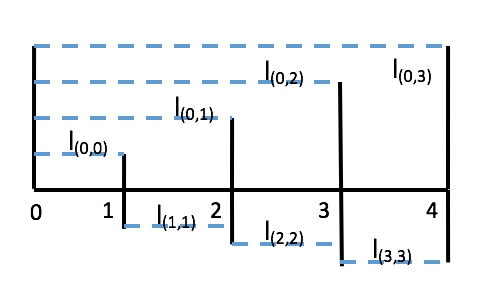
\includegraphics[width=0.4\linewidth]{figtkde/ex11}
\label{example:subfig11}
}
~~\subfloat[(b) Non-overlapping Enumeration]{
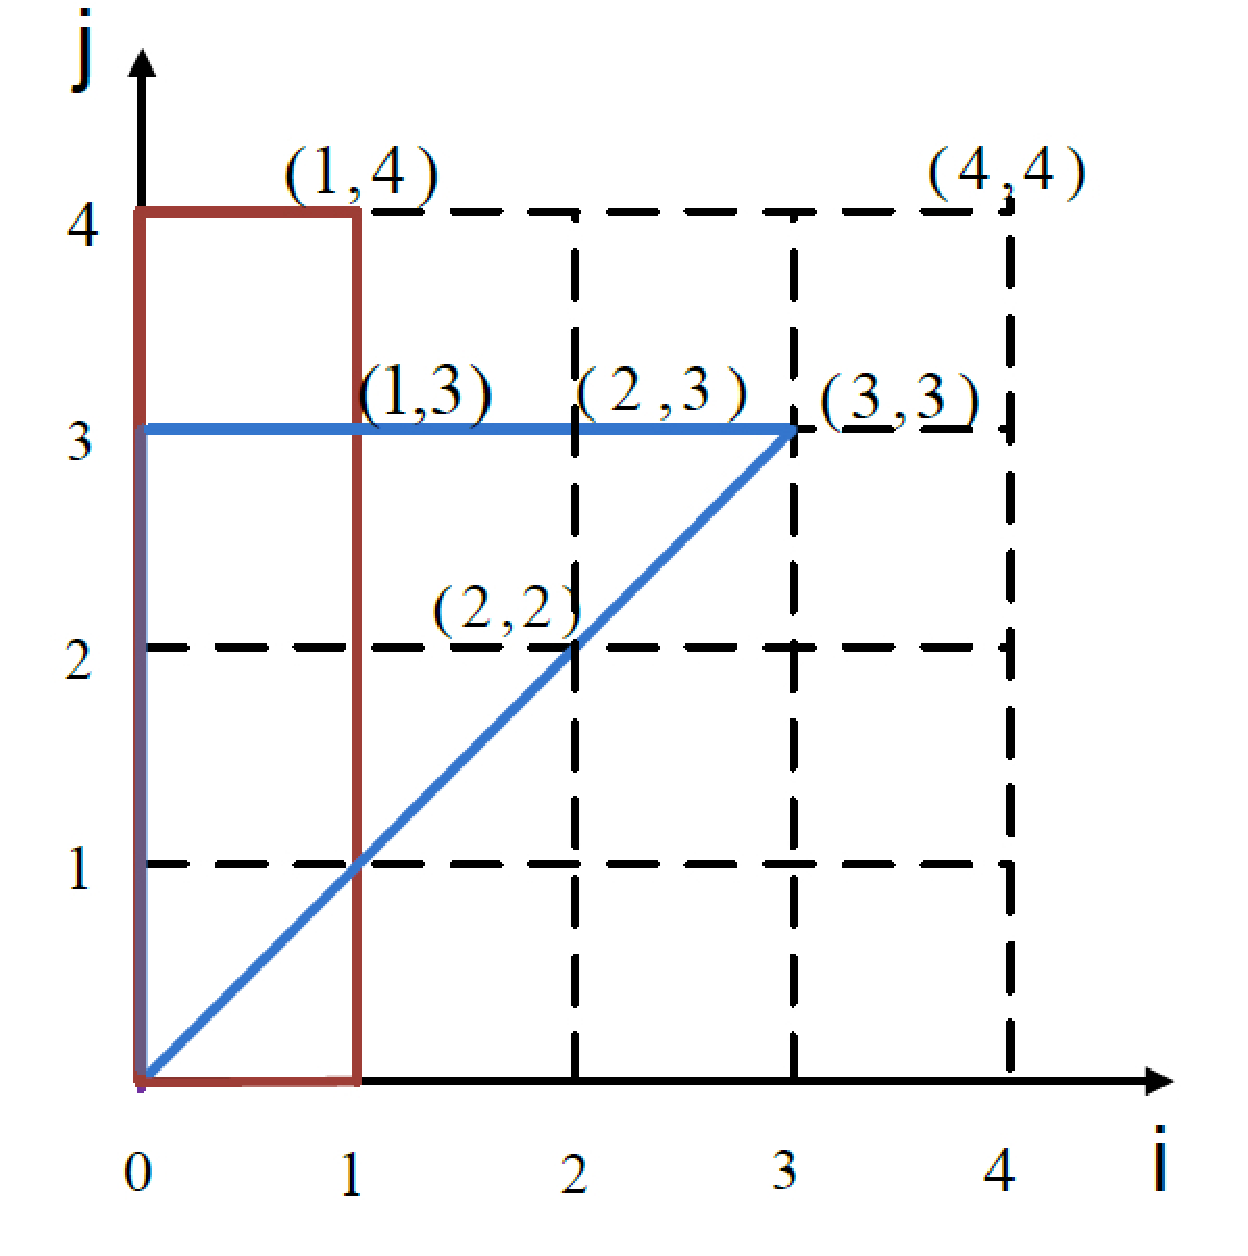
\includegraphics[width=0.3\linewidth]{figtkde/example12}
\label{example:subfig12}
}\\
\caption{Parallel Enumeration Schemes\label{example1}}
\end{figure}

\begin{table}[!ht]
  \centering
  \caption{Example: PU assignment  }\label{exampletable}
  \subfloat[Intervals on PU\label{maptable1}]{
    \centering
\begin{tabular}{|c|c|c|}
	\hline
$Grid$ &$interval_1$ &$interval_2$\\
	\hline
$PU_1$     & $l_{(0,0)}$ & $l_{(0,1)}$\\
	\hline
$PU_2$     & $l_{(1,1})$ & $l_{(1,2)}$\\
	\hline
$PU_3$     & $l_{(2,2)}$& $l_{(2,3)}$\\
    \hline
$PU_4$     & $l_{(3,3)}$& \\
\hline
\end{tabular}
  }
  \subfloat[ Intervals on CPU\label{maptable2}]{
    \centering
   \begin{tabular}{|c|}
	\hline
$intervals$ \\
	\hline
$l_{(0,2)}$ \\
	\hline
$l_{(0,3})$ \\
	\hline
$l_{(1,3)}$\\
\hline
\end{tabular}
}

\end{table}


The aforementioned approach has a few drawbacks: First, non-continuous intervals cannot be processed by parallel units. Hence, there are around $n\cdot {n \choose k}$ (k>2 in above example) intervals that will be processed sequentially by the CPU. Second, some $PUs$ may have fewer number of intervals as a consequence. For example, $PU_4$ has only one interval (i.e. $\{l_{(3,3)}\}$). Hence, the overlapping enumeration parallel strategy causes an unbalanced workload among $PUs$.  Third, for each $PU$, each interval is assigned to a thread. The lengths of intervals are different and this can further creates different workloads among different threads while accumulating statistics for computing $LRT$. To overcome the drawbacks of this approach, the Inclusion-Exclusion parallel strategy is proposed.

\paragraph{Inclusion-Exclusion Parallel Strategy}

For this new scheme, we apply a map-reduce
scheme~\cite{kbest1}~\cite{kbest2} that distributes intervals among parallel
units. The parallel units compute the $k$-best intervals from the
assigned intervals. In the final stage, all $k$-best intervals per
parallel unit are reduced to a single $k$-best list of regions.  To
overcome the issues of the overlapping enumeration scheme, we need to
solve two challenges: First, how can we compute the LRT of a single
interval of a spatial data-grid in $\bigo(1)$. Second, how can we
enumerate intervals so that we can equally distribute them on parallel
units without space and runtime overheads.

The first challenge can be solved by relying on the 1EXP property. For
example, the parameters of the interval $(i,j)$ can be deduced by
having the calculation:

The region $A_j$ counts all the events from the left most data-cell in
the spatial grid to position $j$, i.e., $A_j = I_0 + \ldots +
I_j$. The region $B_i$ counts all the events from the right most
data-cell to position $i$, i.e., $B_i =  I_3 + \ldots +
I_{j}$. The region $G = I_0 + \ldots + I_3$ denotes the whole spatial
grid.
\begin{equation}
I_{ij} = A_j + B_i - G
\end{equation}
For an interval $I_{ij}$, the counts can be deduced by applying the
inclusion/exclusion principle on the set count.  The sum of $|A_i|$ +
$|B_j|$ over-counts the interval by $G$. The computation of $A_j$ and
$B_i$ can be done in linear time, i.e., $\bigo(n)$, as a
pre-computation step. The actual computation of an interval is reduced
to one addition and subtraction, hence, the computation of a single
interval is performed in $\bigo(1)$. In section~\ref{BG}, the property of the log-likelihood statistic (LRT) computation on 1EXP family allows us to simplify to aggregate the events count from a given interval $I$ (denoted as $\sum $). The events count from actual measurement and baseline measurement $m_l,b_l$
are obtained based on $\sum I$ without direct computation of the complement of $I (i.e. \bar I)$. After collecting the aggregated events count of $(m_l,b_l)$, theorem~\ref{thm1} is applied to get the LRT value of interval $I$. In Figure ~\ref{par:subfig1}, it shows four interval composed by five points and counts of $m_l,b_l$ for $I_i$ are shown in Figure ~\ref{par:subfig2}. For example, for interval $I_{13}=A_3+B_1-G$, we can get $m_{13}=(2+2+15)+(2+15+3)-(2+2+15+3)=17$ and $b_{13}=(10+8+20)+(8+6+2)-(10+8+20+2)=28$. From above, we know the LRT value of $l_{(1,3)}$ is calculated as: $lrt_{(1,3)}=m_{13}log(\frac{m_{13}}{b_{13}}+(1-m_{13})log(\frac{1-m_{13}}{1-b_{13}})=17\cdot log(17/28)-16\cdot log(16/27)=-0.11$


 %BFS: Please draw a picture for a single overlap area for A, B and G.
 %for demonstrating the the equations of

 % --------------------->j (for A)
 %        (for B)  i<------------------------
 % <----------------------------------------> (for G)
 %                  <--->  (for Interval (i,j))


% BFS: Explain why the addition/subtraction still works
 %for the LRT computation because of 1EXP
\begin{figure}[t]
\centering
\subfloat[(a) inclusive exclusive strategy for 4 intervals ]{
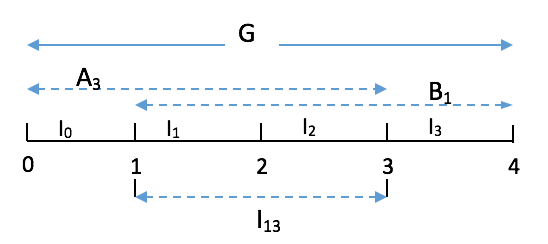
\includegraphics[width=0.4\linewidth]{figtkde/inclusiveex1d.png}
\label{par:subfig1}
}
~~\subfloat[(b) $m_l,b_l$ count for each interval ]{
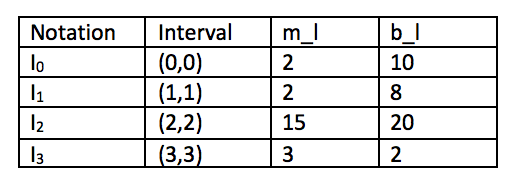
\includegraphics[width=0.4\linewidth]{figtkde/inex1dtable.png}
\label{par:subfig2}
}\\
\caption{Example of Inclusive Exclusive Parallel Strategy\label{inex1d}}
\end{figure}

For balancing the workload, we require that intervals are equally
distributed on parallel units. We solve this problem by enumerating
all intervals from zero onwards.
For our example, we enumerate
intervals and assign each interval a unique number between $0$ and
$\frac{n(n+1)}{2}-1=10$ where $n$ is 4, which we refer to as
\emph{representative number}. By enumerating the intervals we can
easily split the range of the enumeration into equal sub-ranges that
we distribute on the parallel units.  If there are $p$ parallel units
and $\frac{n(n+1)}{2}$ intervals, we achieve a balanced workload with
approximately $\left \lceil \frac{n(n+1)}{2 p} \right\rceil$ intervals
per parallel unit since each interval takes the same constant runtime
to compute.

Let's assume we have 5 parallel units.  parallel unit can process
two intervals at most. Hence, each parallel unit processes exactly 2
intervals. Intervals with representative numbers from $0$ to $1$ are
mapped to the first parallel unit; intervals with representative
numbers from $2$ to $3$ are mapped to the second parallel unit; and so
forth.

The question arises how can we find good representative numbers for
intervals in a spatial data-grid. We could simply enumerate all
intervals exhaustively, assign numbers for each interval on the fly,
and store the representative-number/interval map explicitly.
Unfortunately, the explicit construction of the array map renders to
be expensive in the presence of multi-dimensional large spatial data
grids. A one-dimensional spatial data grid exhibits a the space
worst-case complexity of $\bigo(n^2)$ for computing the map. For a
multi-dimensional spatial data grid, the space worst-case complexity
grows exponential with the number of dimensions, i.e., $\bigo(n^{2k})$
where $k$ is the dimensionality of the spatial data grid. Also, the
map must be shared among all parallel units requiring communication
and memory for storage. To overcome the high storage and communication
costs of the map, we propose a closed-form for mapping representative
numbers to intervals.

If we map each interval $l_{i,j}$ as a point $(i,j)$ and plot these
points onto two-dimensional space, a triangular shape is formed. In
Figure~\ref{example:subfig12}, all of the $10$ intervals in this
example forms a triangle shape enclosed by points
${(0,0),(3,3),(0,3)}$, (i.e. intervals:
${l_{(0,0)},l_{(3,3)},l_{(0,3)}}$).

We notice that the total number of intervals is the product of $(n+1)$
and ${\frac{(n)}{2}}$. A rectangular shape can be formed by this
product: $[width,height]=[n+1,{\frac{n}{2}}]$. In this example,
$\{{(0,0)},{(0,1)},{(1,4)},{(0,4)}\}$ forms a rectangle $R_1$ and it
has the exact same number of points as the formed triangular shape
$R_2$. Therefore, each point in this rectangle can be mapped to one
point in the triangle space.

The closed-form has a runtime and space worst-case complexity of
$\bigo(1)$. The closed-form calculation is divided into two steps:
First, we convert the representative number to a two-digit number
system where the first base $b_0$ is $n$ and the second base $b_1$ is
$\frac{n+1}{2}$. We refer to the two-digits as \emph{Rectangular
  Space}. Given a representative number $r$, the number $r$ is
expressed by $r = d_1 b_0 + d_0$ where $d_1$ and $d_0$ are the digits
of the representative number in the two-digit number system with the
base $b_0$ and $b_1$, respectively. Note that the digit $d_1$ ranges
from $0$ to $\frac{n+1}{2}-1$ and the second digit ranges from $0$ to
$n-1$.  The conversion follows the Horner scheme~\cite{horner} for
number conversion, i.e.,
\begin{align*}
  d_0 &= r\mod n \\
  d_1 &= (r \div n) \mod \frac{n+1}{2}
\end{align*}

In the later section of this work, we refer to the mapping of a
representative number to two digits as $\phi_1$.  The two-digit number
system has exactly $\frac{n(n+1)}{2}$ numbers available. However, the
two digits of a representative number in the two-digit number system
with base $n$ and $\frac{n+1}{2}$ do not represent intervals
yet. There could be numbers whose first digit is larger than the
second digit and vice versa, that would violate the constraints $0
\leq i \leq j < n$.


Hence, we require a further mapping that maps the two digits of a
representative number to intervals.  We refer to the second mapping as
$\phi_2$ in this work. The second mapping suffices the interval
condition,
\begin{equation*}
(d_1, d_0) \mapsto
\begin{cases}
(d_1, d_1 + d_0), & \mbox{if $d_1 + d_0 < n$,} \\
(n - d_1 - 1, 2 n - d_1 - d_0 -1), & \mbox{otherwise.}\\
\end{cases}
\end{equation*}

For our example, we can convert a representative number to the
two-digit number system, subsequently convert the two digits to
intervals as shown in Table~\ref{1dconversion} and ~\ref{2dconversion}.

% BFS: Please put the conversion into a figure.
% BFS: Explain $phi_2$ with two examples. Pick one example for both cases
\begin{table}[t]
\centering \caption{one digit number to two-digit number system\label{tab:op}}
     \begin{tabular}{|c|c|c|c|c|}
	\hline
    0$\rightarrow (0,0)$  &  $1 \rightarrow (0,1)$&  $2 \rightarrow (0,2)$ &$3 \rightarrow (0,3)$ & $4 \rightarrow (0,4)$\\
    \hline
     5$ \rightarrow (1,0)$ & $6\rightarrow (1,1)$  &  $7 \rightarrow (1,2)$&  $8 \rightarrow (1,3)$ & $9  \rightarrow (1,4)$\\
    \hline
\end{tabular}
\label{1dconversion}
\end{table}

\begin{table}[t]
\centering \caption{two-digit system converts to intervals\label{tab:op}}
     \begin{tabular}{|c|c|c|c|c|}
	\hline
    (0,0)$\rightarrow (0,0)$  &  $(0,1) \rightarrow (0,1)$&  $(0,2) \rightarrow (0,2)$ & $(0,3)\rightarrow (0,3)$  &  $(0,4) \rightarrow (3,3)$\\
    \hline
      $(1,0) \rightarrow (1,1)$&  $(1,1) \rightarrow (1,2)$ &$(1,2)\rightarrow (1,3)$ &(1,3)$\rightarrow (2,3)$  &$(1,4) \rightarrow (2,2)$ \\
    \hline
\end{tabular}
\label{2dconversion}
\end{table}
In the above, we know that the number of intervals is treated as the product of $(n+1) $ and $\frac{n}{2}$ to form a rectangular shape. When $n$ is odd, the multiplication of $\frac{n}{2}$ and $(n+1) $ won't produce the exact number of intervals. To generalize, we extend the calculation of number of intervals to $ \lfloor \frac{n+1}{2}\rfloor \cdot (n+1)$. When $n$ is even, $ \lfloor \frac{n+1}{2}\rfloor = \frac{n}{2}$ and exact number of interval can be mapped. When $n$ is odd, the generalized calculation of $ \lfloor \frac{n+1}{2}\rfloor \cdot (n+1)$ is greater than $ \lfloor \frac{n+1}{2}\rfloor \cdot n$ with $\frac{n+1}{2}$. In addition to satisfy the constraints $0\leq i \leq j < n$ , $d_1\leq \frac{n+1}{2}$ is also applied to filter out these more points in the following:

\begin{equation*}
(d_1, d_0) \mapsto
\begin{cases}
(d_1, d_1 + d_0), & \mbox{if $d_1 + d_0 < n$,} \\
(n - d_1 - 1, 2 n - d_1 - d_0 -1), & \mbox{if $(d_1+1)\leq \frac{n+1}{2}$.}\\
\end{cases}
\end{equation*}
 To illustrate the transformation, Figure~\ref{example:subfig1} and ~\ref{example:subfig2} show small examples on how to transform the intervals when having data points $\{O_0,O_1,O_2,O_3,O_4\}$ and $\{O_0,O_1,O_2,O_3,O_4,O_5\}$ respectively. By plotting out all of intervals in first case in Figure~\ref{example:subfig1}, the triangular shaped space is bounded by $\{(0,0), (3,3), (0,3)\}$. And the rectangular shaped space used for transforming to triangular shape is bounded by $\{(0,0),(1,0), (1,4),(0,4)\}$, which is converted by the representative number from  the number of total intervals(i.e. $10$). Similarly, for second case when $n=5$ is odd,  the triangular shaped space is bounded by $\{(0,0),(4,4),(0,4)\}$ and the rectangular shaped space is bounded by $\{(0,0),(2,0),(2,5),(0,5)\}$ by satisfying the constraints in above . Table~\ref{maptable} shows the transformations.

\begin{figure}[h]
\centering
\subfloat[ Grid size n =4 ]{
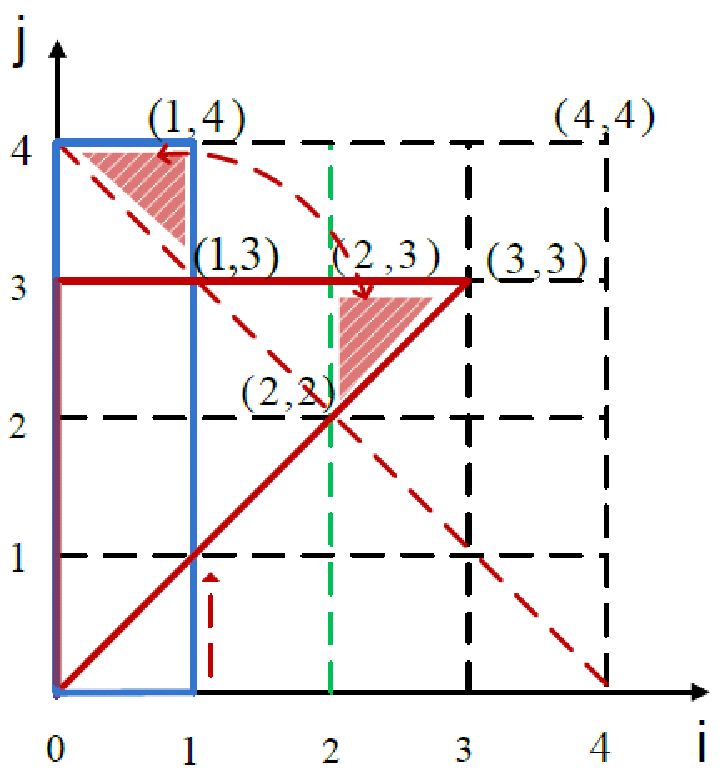
\includegraphics[width=0.25\linewidth]{figtkde/exampleven}
\label{example:subfig1}
}
~~\subfloat[Grid size n =5 ]{
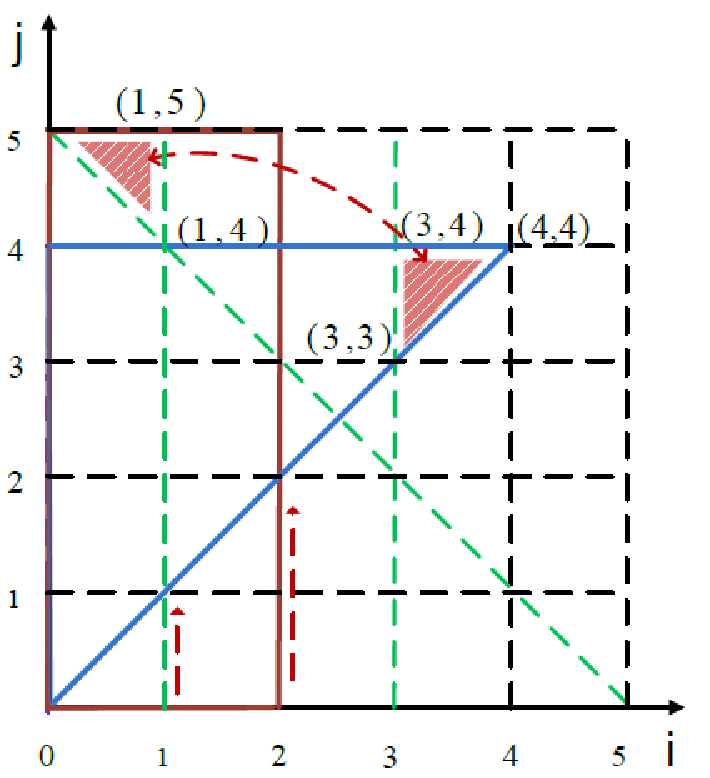
\includegraphics[width=0.25\linewidth]{figtkde/exampleodd}
\label{example:subfig2}
}
\caption{Example: 1-d Interval Transformation}\label{example}
\end{figure}

\begin{table}[!ht]
  \centering
  \subfloat[Grid (4,4)\label{maptable1}]{
    \centering
     \begin{tabular}{|c|c|c|}
	\hline
    (0,0)$\rightarrow (0,0)$  &  $(0,1) \rightarrow (0,1)$&  $(0,2) \rightarrow (0,2)$ \\
    \hline
    (0,3)$\rightarrow (0,3)$  &  $(0,4) \rightarrow (3,3)$&  $(1,4) \rightarrow (2,2)$ \\
    \hline
    (1,3)$\rightarrow (2,3)$  &  $(1,0) \rightarrow (1,1)$&  $(1,1) \rightarrow (1,2)$ \\
    \hline
     (1,2)$\rightarrow (1,3)$  &    &  \\
    \hline

\end{tabular}
  }\\
  \subfloat[Grid (5, 5)\label{maptable2}]{
    \centering
   \begin{tabular}{|c|c|c|}
	\hline
    (0,0)$\rightarrow (0,0)$  &  $(0,1) \rightarrow (0,1)$&  $(0,2) \rightarrow (0,2)$ \\
    \hline
    (0,3)$\rightarrow (0,3)$  &  $(0,4) \rightarrow (0,4)$&  $(0,5) \rightarrow (4,4)$ \\
    \hline
    (1,0)$\rightarrow (1,1)$  &  $(1,1) \rightarrow (1,2)$&  $(1,2) \rightarrow (1,3)$ \\
    \hline
    (1,3)$\rightarrow (1,4)$  &  $(1,4) \rightarrow (3,4)$&  $(1,5) \rightarrow (3,3)$ \\
    \hline
    (2,0)$\rightarrow (2,2)$  &  $(2,1) \rightarrow (2,3)$&  $(2,3) \rightarrow (2,4)$ \\
    \hline
\end{tabular}
  }
  \caption{Example: Interval Transformation for even/odd number of points }\label{maptable}
\end{table}


Therefore, for our proposed strategy, in the first step, we convert the representative number to the
two-digit number system.  In the second step we map the two digits to
an interval. Both steps can be performed with a constant number of
arithmetic operations. Hence, there space and runtime worst-case
complexity of the closed-form is $\bigo(1)$.


\section{Dynamic Pre-computation of Counts for Multi-Dimensional Grids}
\label{sec:dy}
From section~\ref{BG}, we know the log-likelihood statistic (LRT)
computation on 1EXP family is simplified to aggregate the statistic
values from a given region $R$ (denoted as $\sum $). The fraction of
the total from actual measurement and baseline measurement $m_R,b_R$
are obtained based on $\sum R$ without direct computation of the
complement of $R (i.e. \bar R)$. After collecting the aggregated
statistic values $(m_R,b_R)$, theorem~\ref{thm1} is applied to get the
LRT value of region $R$. This property works for any dimensional data grid. 

\subsection{Pre-computation in one-dimension grid}
From section \ref{sec:mov}, we already know inclusive/exclusive precomputation for calculating LRT of intervals can be done in one-dimension grid based on 1EXP property:

\begin{equation}
I_{ij} = A_j + B_i - G
\end{equation},
where interval $A_j$ counts all the events from the left most data-cell in
the spatial grid to position $j$. The interval $B_i$ counts all the events from the right most
data-cell to position $i$ and $G $ denotes counts of the whole spatial
grid.
\subsection{Pre-computation in two-dimension grid}
\begin{figure}[h]
   \tikzset{oo grid/.style={help lines,color=blue!50!black!50,top color=white, opacity=0.5,bottom color=blue!50!black!20, very thick}}
     \begin{center}
     \begin{tikzpicture}

\draw [step=2pt][oo grid](0pt,0pt) rectangle (90pt,90pt);
\draw (10pt,80pt) node {G};
\draw [oo grid](20pt,30pt) rectangle (70pt,60pt);
\draw (45pt,45pt) node {R};

\draw [step=2pt] [oo grid](120pt,0pt) rectangle (210pt,90pt) ;

\draw [step=2pt][oo grid](140pt,30pt) rectangle (190pt,60pt);
\draw [step=2pt][oo grid](120pt,30pt) rectangle (190pt,90pt);
\draw [step=2pt][oo grid](140pt,0pt) rectangle (210pt,60pt);
\draw (130pt,80pt) node {G};
\draw (145pt,70pt) node {A};
\draw (165pt,45pt) node {R};
\draw (130pt,15pt) node {X};
\draw (200pt,75pt) node {Y};
\draw (185pt,15pt) node {B};

\draw (40pt,-15pt) node { (a) Region R in Grid G };
\draw (180pt,-15pt) node { (b) R= $A\cap B$ , $\overline{A}\cap\overline{B} = X \cup Y$};
\end{tikzpicture}
\end{center}
\vspace{-10pt}
\caption{Set Relations for Region Problem}\label{fig:example}
\end{figure}



Consider Figure~\ref{fig:example}(a) showing a rectangular area $R$
embedded in a grid $G$. Instead of counting the number of elements in
$R$ directly, we express set $R$ as set intersections of two sets $A$
and $B$ as shown in Figure~\ref{fig:example}(b). Set $A$ is a
rectangular region that starts in the upper left corner of the grid
and ends at the lower right corner of $R$. Set $B$ is a rectangular
region that starts at the upper left corner of $R$ and ends at the
lower right corner of the grid. Hence, $R=A \cap B$. We denote the
region from the lower left corner of $G$ to the lower left corner of
$R$ by $X$ and the region from the upper right corner of $R$ to the
upper right corner of $G$ by $Y$.

By applying De Morgan's law and inclusion/exclusion principle, the
query of counting the number of elements of region
$R(i_1,j_1,i_2,j_2)$, where $(i_1,j_1)$ is the upper left corner and
$(i_2,j_2)$ is the lower right corner is expressed by (see Proof in
appendix):


\begin{equation}
\label{EQ:precomp}
\begin{split}
|R(i_1,j_1,i_2,j_2)|& = |A(i_2,j_2)| + |B(i_1,j_1)| + |X(i_1,j_2)|  + |Y(i_2,j_1)| - |G|
\end{split}
\end{equation}
\normalsize From Equation ~\ref{EQ:precomp}, we can see that a query
time of $\bigo(1)$ can be achieved by pre-computing statistics of sets
$A$, $B$, $X$, and $Y$ for all possible regions in $G$. Since one of
the corner of $A$, $B$, $X$, and $Y$ is fixed, we can pre-compute the
cardinalities of these sets in tables of size $\bigo(n^2)$.

This pre-computation scheme has been implemented in~\cite{apweb} and
we will give more details and related algorithms in the following.

%BFS: We need to generalize to the multi-dimensional case here!
\subsection{Pre-computation in Multi-dimension grid}
Similarly, this  pre-computation strategy can be extended to multi-dimension grid.
\begin{equation}
\label{EQ:precomp}
\begin{split}
|R(i_1,j_1,...,g_1,...,i_k,j_k,...,g_k)|& = |A(i_k,j_k,...,g_k)| + |B(i_1,j_1,..,g_1)| + \sum |X(i_p,j_q,...,g_r)| - |G|
\end{split}
\end{equation}
where $p,q,...,r$ are the intersect positions of region $R$  and  $1\leq p,q,r \leq k $. $(i_1,j_1,...g_1)$ and  $(i_k,j_k,...g_k)$ are corners of the $k$-dimensional grid. 

\subsection{Implementation of Pre-computation in two-dimension grid}
In the following, we show the detail of the precomputation scheme in two-dimensional grid. This novel and unique approach based on the Inclusive/Exclusive principle and
dynamic programming accumulates the statistic of a region $R$. We build a table in time $\bigo(n^2)$ and then compute the statistic of any region $R$ in $\bigo(1)$ time.

To obtain a query time of $\bigo(1)$, we need to pre-compute sets $A$, $B$, $X$, and $Y$ for all possible regions in $G$. Since one of the corner is fixed we can pre-compute the cardinalities of these sets in tables of size $\bigo(n^2)$.

To obtain the tables for $A$, $B$, $X$, and $Y$, we employ dynamic programming. The dependency and statistic counts' propagation of rows and columns for these tables are shown in Figure~\ref{prec:subfig1},~\ref{prec:subfig2},~\ref{prec:subfig3} and ~\ref{prec:subfig4}. For example, the table for $A$ can be computed using the following recurrence relationship:


\begin{eqnarray}
|A(i,j)|  &= |A(i,j-1)| + |A(i-1,j)| - |A(i-1,j-1)|  + |G(i,j)|
\end{eqnarray}
\normalsize
where $|G(i,j)|$~\footnote{(i,j) represents $(x_i,x_j)$ for simplicity.}counts whether there is an element in the cell location $(i,j)$. The first element and the first column and row need to be populated (initialized) so that all cardinalities of $A$ can be computed. The counts in the remaining rows and columns are accumulated through the dependency of the previous row and column. Figure~\ref{prec:subfig1} shows the computation of set $A$ and the implementations of it is listed in Algorithm~\ref{preinex} (see the proofs and the rest implementation of set $B,X,Y$ in Appendix.)\\

Similarly, the computation of set $B,X,Y$ is listed as the following:

\begin{eqnarray}
|B(i,j)|  &= |B(i+1,j)| + |B(i,j+1)| - |B(i+1,j+1)| + |G(i,j)|
\end{eqnarray}
\normalsize

\begin{eqnarray}
|X(i,j)|  &= & |X(i,j+1)| + |X(i-1,j)| - |X(i-1,j+1)| + |G(i,j)|
\end{eqnarray}
\normalsize

\begin{eqnarray}
|Y(i,j)|  &= & |Y(i+1,j)| + |Y(i,j-1)| - |Y(i+1,j-1)| + |G(i,j)|
\end{eqnarray}
\normalsize

\begin{figure}[h]
\centering
\subfloat[Pre-computation of set A  ]{
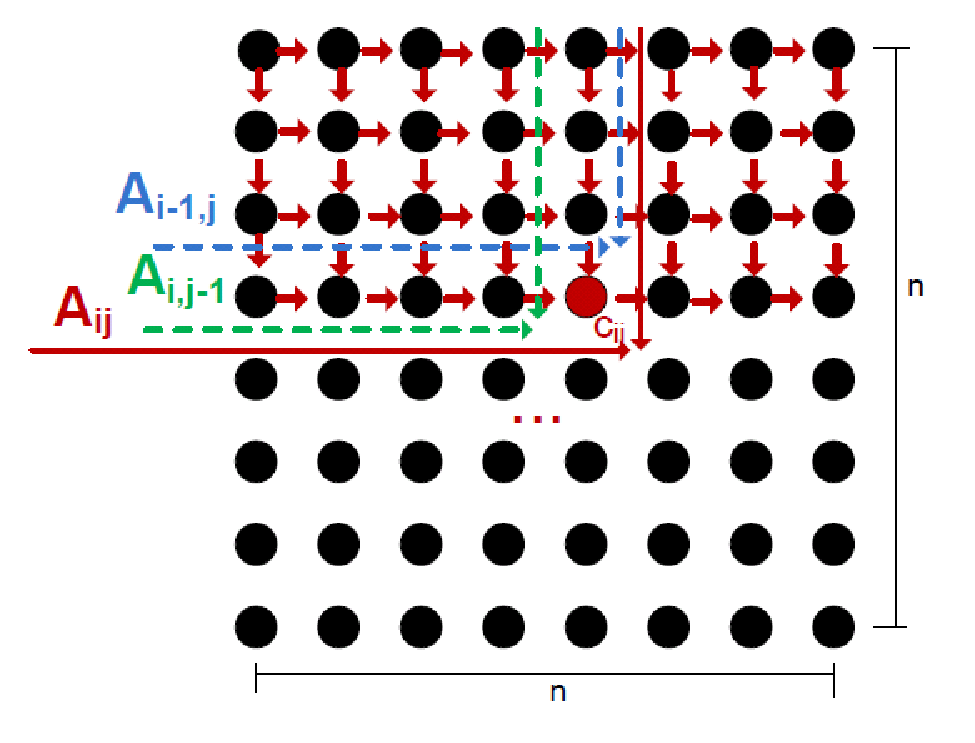
\includegraphics[width=0.25\linewidth]{figtkde/prea}
\label{prec:subfig1}
}
~~\subfloat[Pre-computation of set B]{
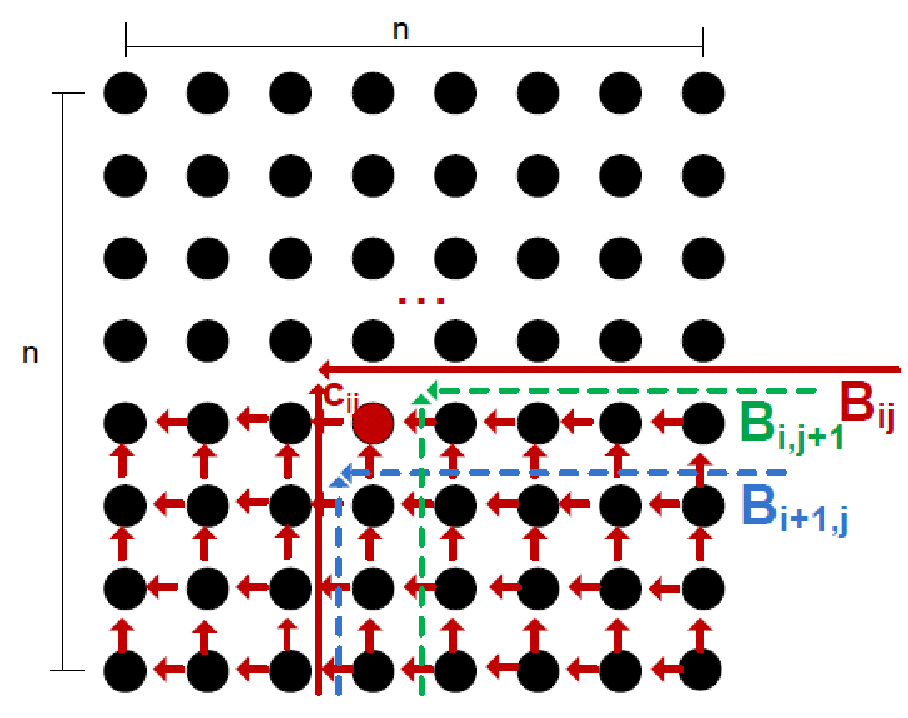
\includegraphics[width=0.25\linewidth]{figtkde/preb}
\label{prec:subfig2}
}\\
~~\subfloat[Pre-computation of set X]{
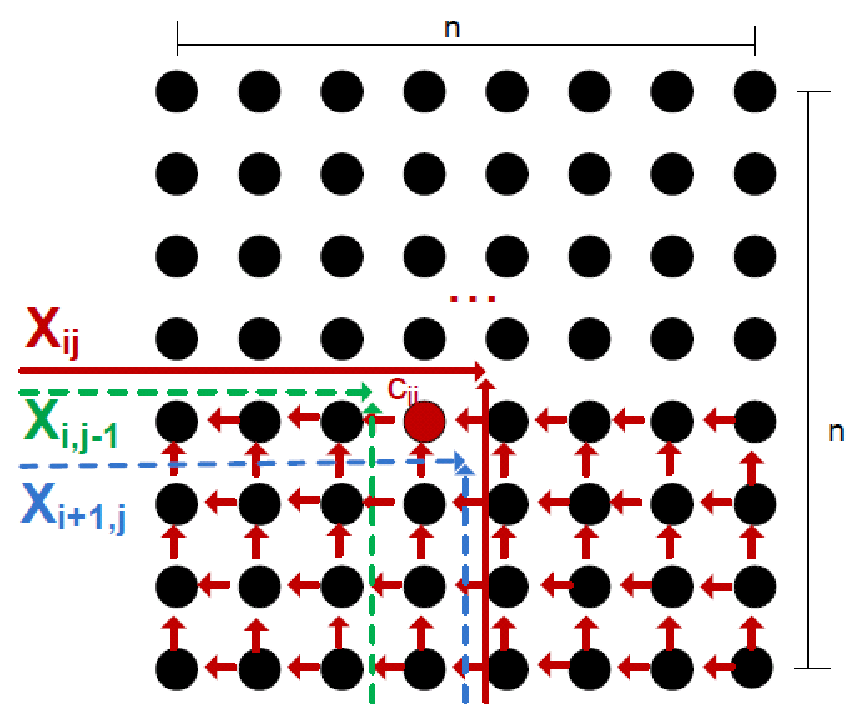
\includegraphics[width=0.25\linewidth]{figtkde/prex}
\label{prec:subfig3}
}
~~\subfloat[Pre-computation of set Y]{
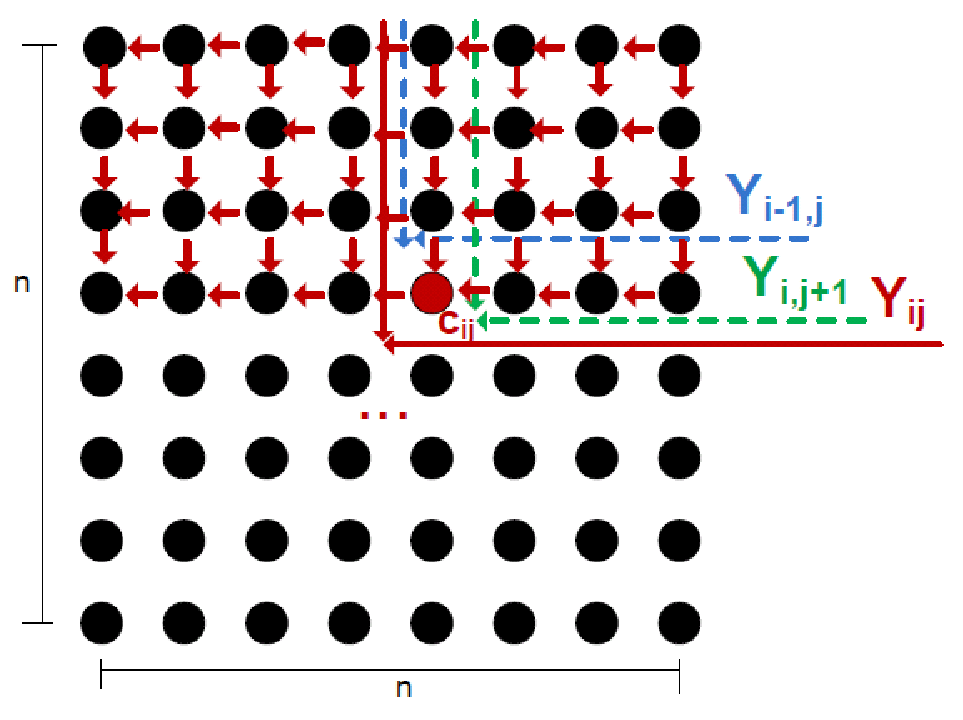
\includegraphics[width=0.25\linewidth]{figtkde/prey}
\label{prec:subfig4}
}
\caption{pre-computation of set A, B, X and Y}\label{prec}
\end{figure}

Due to the high dependency among rows and columns, pre-computing is hard to parallelise and the computation is very fast on a CPU. In our work, the pre-computation of set $A, B, X, Y$ is done on a CPU.

\begin{algorithm}[t!]
\caption{Inclusive/Exclusive Pre-computation for Set A}\label{preinex}
Input: data grid (G) \\
Output: accumulated counts $A(i,j)$\\
------------------------------------------------------------------ \\
\begin{algorithmic}[1]
\State //Initialize first element $A(0,0)$
\State {\textit { $A(0,0)$\(\leftarrow\)$G(0,0)$}}
\State //accumulation of remaining elements in first row
\For {\textit  j\(\leftarrow\)1 to \textit{n}}
\State{\textit { $A(0,j)$ \(\leftarrow\) $G(0,j)$ +$A(0,j-1)$}}
\EndFor
\State //accumulation of remaining elements in first column
\For{\textit  i\(\leftarrow\)1 to \textit{n}}
\State  {\textit {$A(i,0)$\(\leftarrow\)$G(i,0)$ + $A(i-1,0)$}}
\EndFor
\State //accumulation of all the elements in remaining rows and columns
\For{\textit  k\(\leftarrow\)1 to \textit{n}}
\For{\textit  i\(\leftarrow\)k to \textit{n}}
\State  {\textit { $A(i,k)$\(\leftarrow\) $G(i,n+k)+A(i-1,k)+A(i,k-1)-A(i-1,k-1)$}}
\EndFor
\For{\textit  j\(\leftarrow\)k to \textit{n}}
\State  {\textit { $A(k,j)$\(\leftarrow\) $G(k,n+j)+A(k,j-1)+ A(k-1,j)-A(k-1,j-1)$}}
\EndFor
\EndFor
\end{algorithmic}
\end{algorithm}


\section {Range Mapping Scheme} \label{RMS}
In this section, we study how parallelism helps to enumerate all of the rectangular regions (R) in a spatial grid (G). We will explain this scheme in one-dimensional, two-dimensional, and $k$-dimensional data-grids.

From section~\ref{sec:mov1}, we know that if all of the pairwise intervals between $n+1$ data points, denoted as $l_{(i,j)}$, are plotted as point $(i,j)$ onto two-dimensional coordinate system, they form triangular shape. Each pair of $(i,j)$ in triangular-shaped space can be transformed to pair $(i',j')$ in rectangular-shaped space. After transformation, it enables the whole rectangular space to be partitioned into equal portions. Each portion consists of same amount of pairs and is distributed onto different ``parallel computing component'' (PU) to balance workload and facilitate parallelization. We name this transforming scheme as range mapping scheme. This scheme can be directly extended to two dimensional spatial grid and multi-dimensional grid.

Figure~\ref{trans:subfig1} plots out all of the intervals $l_{(i,j)}$ in two-dimensional space and we can see that these points $(i,j)$ forms a triangle. Figure~\ref{trans:subfig2} shows the rectangular-shaped space after transformation.

\begin{figure}[h]
\centering
\subfloat[]{
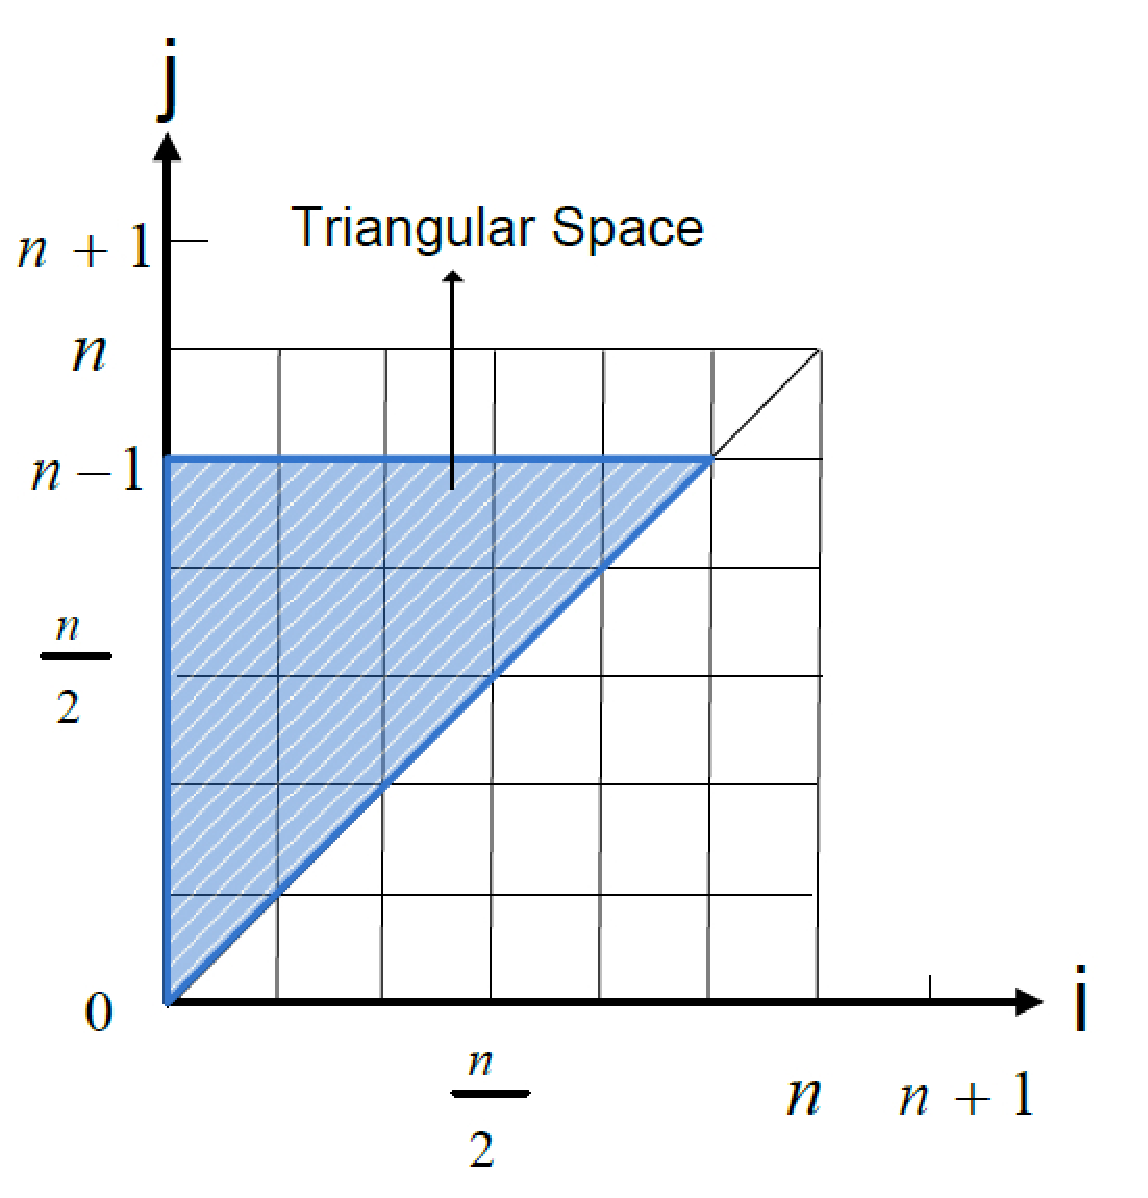
\includegraphics[width=0.35\linewidth]{figtkde/range1}
\label{trans:subfig1}
}
~~\subfloat[]{
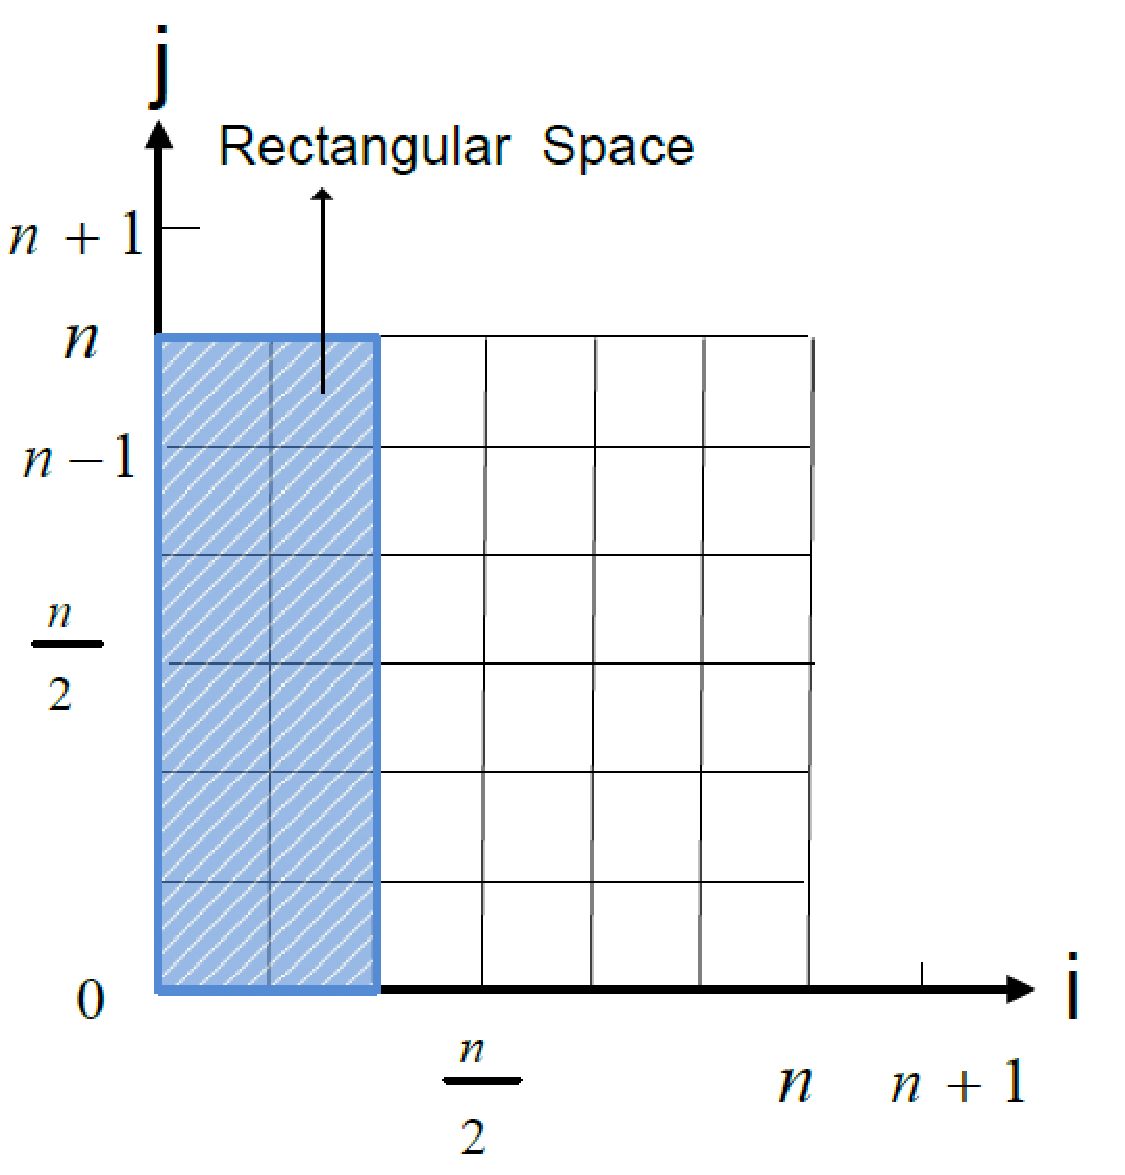
\includegraphics[width=0.35\linewidth]{figtkde/range2}
\label{trans:subfig2}
}
\caption{1-d Interval Transformation from $[n,n]$ to $[(n+1)/2,n]$}\label{modelBF}
\end{figure}

To assign an interval $l_(i,j)$ to a $PU_y$, Horner scheme discussed above is applied~\cite{horner}. Then transform $(i,j)$ from rectangular space to $(i',j')$  to triangle space. We give details in the following:

\subsection{One-Dimensional Mapping}
For one-dimensional range mapping scheme, we assume there are $n$ data points, therefore having ${\frac{n \cdot (n+1)}{2}}$ intervals. There are two cases in one-dimensional grid: (1) The grid size $n$ is even (2) The grid size $n$ is odd. \\

Given the following information:
\begin{eqnarray}
& N = \{0,...,n\}               & \\
& R = \{(i,j)\in [0,...,\lfloor \frac{n+1}{2}\rfloor -1] \times [0,...,n]\}     &\\
& T = \{(i',j') \in [0,...,n] \times [0,...,n] | i'<=j'\}   &\\
& M = \{0,..., \lfloor \frac{n+1}{2}\rfloor \cdot (n+1)-1\}  &\\
\end{eqnarray}
where  $ N$ is the set of $n+1$ data points which partitions one-dimensional grid into $n$ intervals. $ R$ is the rectangular space formed by $\{[0,...,\lfloor \frac{n+1}{2}\rfloor -1]\times [0,...,n]\}$ and each point $(i,j)$ (i.e. interval) in this space is assigned to a certain $PU_y$. $T$ is the triangular space formed by original intervals, where each interval is $l_(i',j')$ $(0<i'<j'\leq n)$. $ M$ is total number of  intervals for computing $LRT$.\\
 To have a generalized form of the mapping scheme when grid size $n$ is even or odd , we extend the calculation of total intervals from $\frac{n+1}{2} \cdot n$ to $\lfloor \frac{n+1}{2}\rfloor \cdot (n+1)$. When $n$ is even, we know $\lfloor \frac{n+1}{2}\rfloor =\frac{n}{2}$. When $n$ is odd, we know $\lfloor \frac{n+1}{2}\rfloor= \frac{n+1}{2}$. The generalized computation of number of total intervals in our range mapping scheme is $\frac{n+1}{2} \cdot (n+1) $ no matter grid size $n$ is even or odd, this produces $\frac{n+1}{2}$ more intervals with enlarged set when $n$ is odd but have exact calculation when $n$ is even. \\

\noindent   \textbf{\emph{(1) The grid size $n$ is even:}} A mapping Function $\phi:  M \rightarrow  R \rightarrow  T$  is composed of two functions: $\phi_1:  M \rightarrow  R$ and $\phi_2:  R \rightarrow  T$. Firstly, $\phi_1$ transforms the index value of $y\in  M$ of a certain $PU_y$ to a pair $(i,j)\in  R$ in rectangular space. Secondly, $\phi_2$ transforms the pair $(i,j)\in  R$ from rectangular space to a pair $(i',j')\in  T$ to triangular space.\\
\noindent\begin{definition}
IR Mapping Function
\begin{flalign*}
&&\phi_1:&   M \rightarrow  R & \\
&&y &\mapsto (i,j)
\end{flalign*}
 where $i  = y / (n+1)$ and $j = y \mod (n+1)$.
\end{definition}
IR (Index to rectangular) mapping function assigns a point $(i,j)$ in rectangular space $R$ to $y$ of $PU_y$  by applying inverse horner scheme, where $y\in \{0,...,\lfloor \frac{n+1}{2}\rfloor \cdot (n+1)-1\}$. When $n$ is even, $\lfloor \frac{n+1}{2}\rfloor=\frac{n}{2}$. Point $(i,j)$ is computed by $i  = y / (n+1)$ and $j = y \mod (n+1)$ , where $y$ is the index of a particular $PU$ and constant value of $n$ is the total number of data points in one-dimensional grid.
 \vspace{5mm}
\begin{lemma}
Mapping function $\phi_1$ transforms $y\in M$ (i.e. $y\in \{0,..., \frac{n\cdot (n+1)}{2} -1\}$) to $(i,j) \in R$, where $i \in \{0,...,\frac{n}{2}-1\}$ and $j \in \{0,...,n\}$.
\end{lemma}
When $n$ is even, we know ${\lfloor \frac{n+1}{2}\rfloor} = \frac{n} {2}$. Since $y\in M$ and size of $M$ is equal to $ \frac{n}{2} \cdot n$, it is obviously seen that $i\in \{0,...,\frac{n}{2}-1\}$ when $i  = y / (n+1)$. Similarly, $j\in \{0,...,n\}$ when $j = y \mod (n+1)$.
\vspace{5mm}
\begin{lemma}
Mapping function $\phi_1:   M \rightarrow  R, y \mapsto (i,j)$ is bijective.
\end{lemma}
 In one-dimension grid, for each $PU_y$, we can denote $y=i\cdot n+j$, where $y \in \{0,...,{\frac{n \cdot (n+1)}{2}}\}$ and $0\leq i, j < n$. From the horner scheme, we know lemma 1 produces one-to-one mapping from $y$ to $(i,j)$. At the same time, given $(i,j)$, $y$ can be uniquely constructed as $y=i\cdot n+j$. Therefore, $y \mapsto (i,j)$ is bijective.
\vspace{5mm}

\begin{definition}
RT Mapping Function
\begin{eqnarray}
&\phi_2:&   R \rightarrow  T  \\
&(i,j)& \mapsto (i',j')=
  \begin{cases}
   (i,i+j) & \text{if } (i+j) < n \\
   (n-i-1,2n-i-j-1)) & \text{otherwise}
  \end{cases}
\end{eqnarray}
\end{definition}
RT (rectangular to triangular) mapping function transforms point $(i,j)$ in rectangular space to point $(i',j')$ in triangular space shown in above equation. This transformation is achieved by satisfying the constraints: $(i,j)\in \{[0,...,\lfloor (n+1)/2] \times [0,...,n]\}$ and $0\leq i' \leq j'<n$. To fulfill this constraint, line $i+j=n$ divide the rectangular space into two sub-spaces: (a) $i+j<n$, (b) $i+j\geq n$. In (a), transformed point $(i',j')$ is calculated as $(i,i+j)$ . In (b), transformed point $(i',j')$ is calculated as $(n-i-1,(n-i-1)+(n-j))$ (i.e. $(n-i-1,2n-i-j-1)$). It is clearly seen that $(i',j')$ satisfies $0\leq i' \leq j'<n$ after transformation. Figure~\ref{even:subfig1} visualizes the mapping.

\vspace{5mm}
\begin{lemma}
Mapping function $\phi_2$ transform $(i,j) \in R$ to $(i',j')\in T $, where $i' \in \{0,...,n\}$ and $j' \in \{0,...,n\}$.
\end{lemma}
It is true that $i<n$ and $n-i-1<n$. Also when $(i+j) < n$ and $j'=i+j$, we can get $i'\leq j'<n$. When $(i+j) \geq n$, we get $i'\leq j'=2n-i-j-1=(n-i)+(n-j-1)<n$. Therefore,$i' \in \{0,...,n\}$, $j' \in \{0,...,n\}$ and $i'\leq j'$.
\vspace{5mm}
\begin{lemma}
Mapping function $\phi_2:   R \rightarrow  T,y \mapsto (i,j)$ is bijective.
\end{lemma}
From above definition, we see that each $(i,j)$ uniquely maps to $(i',j')$. We get $i'=i, j'=i+j$ when $i+j<n$. And we get $i'=n-i-1, j'=2n-i-j-1$ when $i+j\geq n$. Correspondingly,  given $(i',j')$, $(i,j)$ can be uniquely obtained by $i=i', j=j'-i'$ or $i=n-i'-1, j=i'+n-j'$. Therefore, $y \mapsto (i,j)$ is bijective.
\vspace{5mm}
\begin{corollary}
The function $\phi:   M  \rightarrow R \rightarrow  T,y \mapsto (i',j')$ is bijective.
\end{corollary}
Since $M  \rightarrow R$ and $R \rightarrow  T$ are bijective respectively, this means $y \mapsto (i,j)$ and $(i,j) \mapsto (i',j')$ are bijective. Therefore $ M  \rightarrow R \rightarrow  T$,  $y \mapsto (i',j')$ is bijective.
\vspace{5mm}

\noindent \textbf{\emph {(2) The grid size $n$ is odd:}} Function $\phi:  M \rightarrow  R \rightarrow  T$ is composed of two mapping functions: $\phi_1:  M \rightarrow  R$ and $\phi_2:  R \rightarrow  T$. Firstly, $\phi_1$ transforms the index value of $y\in  M$ of a certain $PU_y$ to a pair $(i,j)\in  R$ in rectangular space. Secondly, $\phi_2$ transforms  $(i,j)\in  R$ from rectangular space to a pair $(i',j')\in  T$ in triangular space.
\vspace{5mm}
\noindent\begin{definition}
IR Mapping Function
\begin{eqnarray}
\phi_1:   M \rightarrow  R & \\
y \mapsto (i,j)
\end{eqnarray}
 where  $i  = y / (n+1)$ and $j = y \mod (n+1)$.\\
 IR (Index to rectangular) mapping function assigns a point $(i,j)$ in rectangular space $R$ to $y$ of $PU_y$  by applying inverse horner scheme, where $y\in \{0,...,\lfloor \frac{n+1}{2}\rfloor \cdot (n+1)-1\}$.  Point $(i,j)$ is computed by $i  = y / (n+1)$ and $j = y \mod (n+1)$ , where $y$ is the index of a particular $PU$ and constant value of $n$ is the total number of data points in one-dimensional grid. Since $n$ is odd in this case, there has $\frac{n+1}{2}$ more data points (intervals) in the extended form than the original total number of intervals and they  won't be processed.
\end{definition}
 \vspace{5mm}
\begin{lemma}
Mapping function $\phi_1$ transforms $y\in M$ to $(i,j) \in R$, where $i \in \{0,...,\frac{n+1}{2}-1\}$ and $j \in \{0,...,n\}$.
\end{lemma}
When $n$ is odd, we know $ {\lfloor \frac{n+1}{2}\rfloor} = {\frac{n+1}{2}}$.  Since $y\in M$ and size of $M$ is extend to $  \frac{n+1}{2} \cdot (n+1)$ , we can derive that $i\in \{0,...,\frac{n+1}{2}-1\}$ when $i  = y / (n+1)$. Similarly, $j\in (0,n)$ when $j = y \mod (n+1)$.
\vspace{5mm}
\begin{lemma}
Mapping function $\phi_1:   M \rightarrow  R,y \mapsto (i,j)$ is bijective.
\end{lemma}
 In one-dimension grid, for each $PU_y$, we can denote $y=i\cdot (n+1)+j$, where $y \in (0,{\frac{(n+1) \cdot (n+1)}{2}})$ and $0\leq i, j < n$. From the horner scheme and the quotient-remainder theorem , we know there is unique mapping from $y$ to $(i,j)$. Correspondingly, given $(i,j)$, $y$ can be uniquely constructed as $y=i\cdot (n+1)+j$. Therefore, $y \mapsto (i,j)$ is bijective.
\vspace{5mm}
\begin{definition}
Mapping Function
\begin{eqnarray}
&\phi_2:& R\rightarrow T\\
&(i,j)&\mapsto (i',j')=
  \begin{cases}
   (i,i+j) &\text {if } (i+j) < n \\
   (n-i-1,2n-i-j-1) & \text {if}(i+1) \leq \frac{(n+1)}{2}
  \end{cases}
\end{eqnarray}
\end{definition}
RT (rectangular to triangular) mapping function transforms point $(i,j)$ in rectangular space to point $(i',j')$ in triangular space shown in above equation. This transformation is achieved by satisfying the constraints: $(i,j)\in \{[0,...,\lfloor (n+1)/2] \times [0,...,n+1]\}$ and $0\leq i' \leq j'<n$. To fulfill this constraint, line $i+j=n$ divide the rectangular space into two sub-spaces: (a) $i+j<n$, (b) $i+j\geq n$. Furthermore, when $n$ is odd, we have $\frac{(n+1)}{2}$ more points than needed and thus the rectangular shape is enlarged, the constraint of $(i+1) \leq \frac{(n+1)}{2}$ is applied to limit the unnecessary transformation of points in rectangular space to triangular space. To explain this, when line $i+j=n$ intersection with line $(i+1) = \frac{(n+1)}{2}$, we can get $j=n-i=n-\frac{(n+1)}{2}+1=\frac{(n+1)}{2}$. Hence when $i+j<n$, the unnecessary points above the the intersection point on the line of $(i+1) = \frac{(n+1)}{2}$ are filtered out.  In (a), transformed point $(i',j')$ is calculated as $(i,i+j)$ . In (b), transformed point $(i',j')$ is calculated as $(n-i-1,(n-i-1)+(n-j))$ (i.e. $(n-i-1,2n-i-j-1)$). This mapping strategy shows that $(i',j')$ satisfies $0\leq i' \leq j'<n$ after transformation. Figure~\ref{odd:subfig1} visualizes the mapping.
\vspace{5mm}
\begin{lemma}
Mapping function $\phi_2:   R \rightarrow  T$ transform $(i,j) \in R$ to $(i',j')\in T $, where $i' \in \{0,...,n\}$ and $j' \in \{0,...,n\}$ in triangular space.
\end{lemma}
It is true that $i<n$ and $n-i-1<n$. Also when $(i+j) < n$ and $j'=i+j$, we can get $i'\leq j'<n$. When $(i+j) \geq n$, we get $i'\leq j'=2n-i-j-1=(n-i)+(n-j-1)<n$. Moreover, the constraint of $(i+1) \leq \frac{(n+1)}{2}$ is applied to limit the unnecessary transformation of points when $n$ is odd. Therefore,$i' \in \{0,...,n\}$, $j' \in \{0,...,n\}$ and $i'\leq j'$ in triangular space.
\vspace{5mm}
\begin{lemma}
Mapping function $\phi_2:   R \rightarrow  T, (i,j) \mapsto (i',j')$ is injective.
\end{lemma}
From above mapping strategy, we see that each $(i',j')$ has single mapping to $(i,j)$ and some unnecessary $(i,j)$ are not processed due to $R$ is enlarged. There has $i'=i, j'=i+j$ when $i+j<n$. And there has $i'=n-i-1, j'=2n-i-j-1$ when $i+j\geq n$. There is no over-lapping mapped point $(i',j')$ based on the constraint of $i+j<n$ and  $(i+1) \leq \frac{(n+1)}{2}$. Correspondingly, given $(i',j')$, $(i,j)$ can be obtained by $i=i', j=j'-i'$ or $i=n-i'-1, j=i'+n-j'$. However, due to $R$ is enlarged space , $(i,j) \mapsto (i',j')$ is injective when $n$ is odd.
\vspace{5mm}
\begin{corollary}
Mapping function $\phi:   M \rightarrow R \rightarrow  T,y \mapsto (i',j')$ is injective.
\end{corollary}
From above, we know $M  \rightarrow R$ (i.e. $y \mapsto (i,j)$) is bijective and $R \rightarrow  T$ (i.e. $(i,j) \mapsto (i',j')$) is injective. Therefore $ M  \rightarrow R \rightarrow  T$,  $y \mapsto (i',j')$ is injective.

Figure~\ref{even:subfig1} and Figure~\ref{odd:subfig1} show the solutions and implementation is shown in Algorithm~\ref{RM}.

\begin{figure}[h]
\centering
\subfloat[ (a) Solution when Grid size n is even number ]{
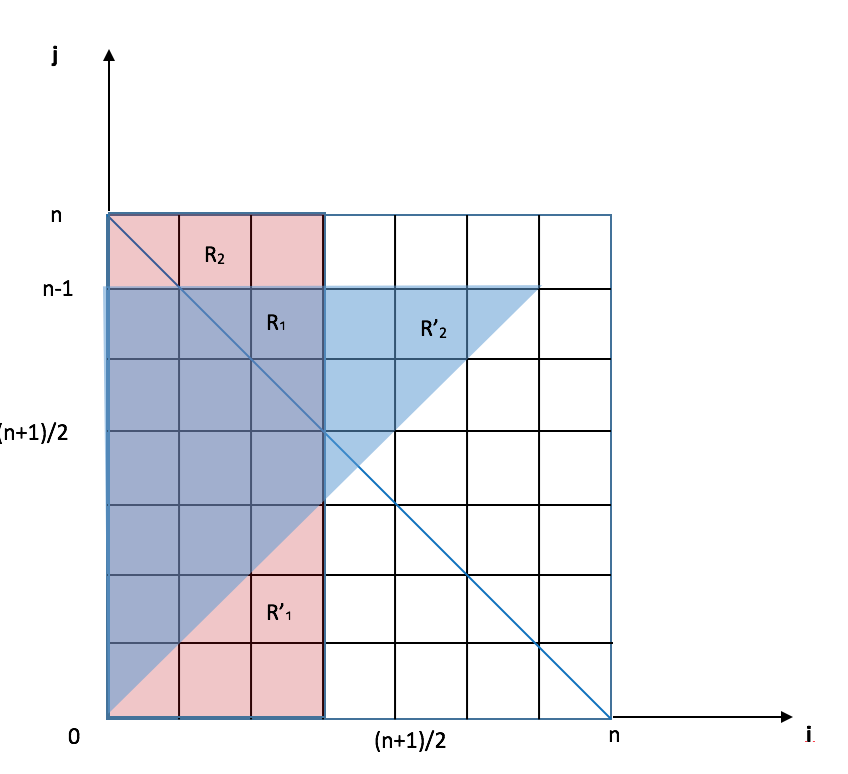
\includegraphics[width=0.35\linewidth]{figtkde/solution1}
\label{even:subfig1}
}
~~\subfloat[ (b) Solution when Grid size n is odd number ]{
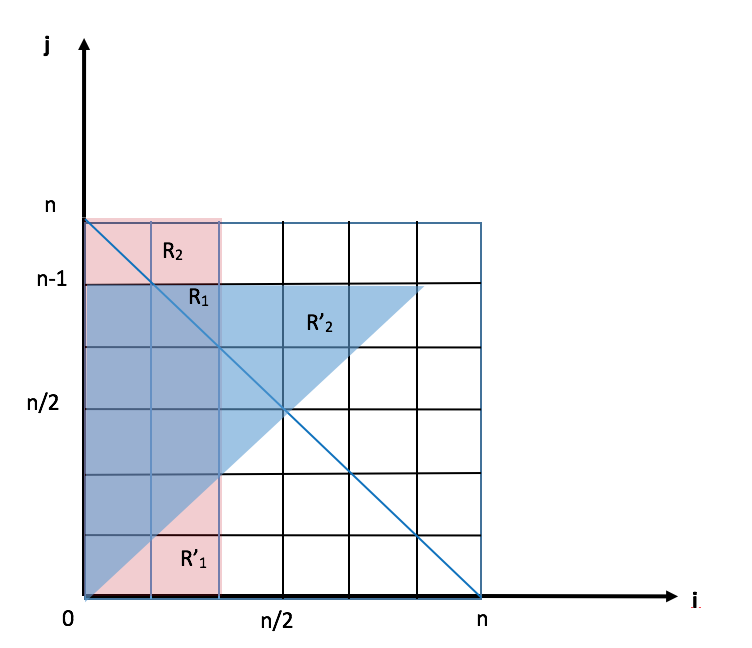
\includegraphics[width=0.35\linewidth]{figtkde/solution2}
\label{odd:subfig1}
}
\caption{1-d Interval Transformation from $[n,n]$ to $[\lfloor (n+1)/2 \rfloor,n+1]$}\label{modelBF}
\end{figure}


\subsection{Two-Dimensional Mapping}
Two-dimensional mapping is extended from one-dimensional mapping directly.
\\Given:
\begin{eqnarray}
& N^2 = N_1\times N_2= \{0..n_1\} \times \{0..n_2\} & \\
& R^2 = R_1 \times R_2=\{(i_1,j_1), (i_2,j_2)\}\in \{[0..\lfloor \frac{n_1+1}{2}\rfloor-1] \times [0..n_1], [0..\lfloor \frac{n_2+1}{2}\rfloor-1] \times [0..n_2]\}&\\
& T^2 =T_1\times T_2=\{(i'_1,j'_1),(i'_2,j'_2)\}\in \{ [0,...,n_1]^2, [0,...,n_2]^2\}  | i'_{1,2}<=j'_{1,2}&\\
& M^2 = \{0.. \lfloor {\frac{n_1+1)}{2}\rfloor}\cdot \lfloor {\frac{n_2+1}{2}\rfloor \cdot (n_1+1)\cdot (n_2+1)}\}&\\
\end{eqnarray}
where $\{N_1,N_2\}$ are set of two dimensional data points with size of $(n_1+1, n_2+1)$ to partition the data grid into $n_1\cdot n_2$ independent cells. $\{R_1, R_2\}$ is rectangular space formed by cell $\{(i_1,j_1), (i_2,j_2)\}$ and each such cell is assigned to a certain $PU_y$ ($y\in M^2$). $\{T_1,T_2\}$ is triangular space formed by original cell $\{(i'_1,j'_1), (i'_2,j'_2)\}$, ($0<i'_1<j'_1\leq n_1,0<i'_2<j'_2\leq n_2\} $)in two dimensional grid. $M^2$ is the total number of cells for computing LRT in  two-dimension grid. Similar as one dimensional grid, we generalize the range mapping scheme by extending the calculation of total cells to $\lfloor {\frac{n_1+1)}{2}\rfloor}\cdot \lfloor {\frac{n_2+1}{2}\rfloor \cdot (n_1+1)\cdot (n_2+1)}$ when either $n_1$ or $n_2$ is odd or even. In the following definitions and lemmas, we won't differentiate the scenario of even and odd number of partitions since we already shown the capability of our generalized form in one dimensional grid.  \\

\noindent\begin{definition}
IR Mapping Function
\begin{flalign*}
&&\phi_1:&   M^2 \rightarrow  R^2 & \\
&&y &\mapsto (i_1,j_1)\times (i_2,j_2)
\end{flalign*}
 where $i_1 \in \{0,...,\lfloor {\frac{n_1+1)}{2}\rfloor}-1\}$ , $j_1 \in \{0,...,n_1\}$ and $i_2 \in \{0,...,\lfloor {\frac{n_2+1)}{2}\rfloor}-1\}$ , $j_2 \in \{0,...,n_2\}$.
\end{definition}
IR (Index to rectangular) mapping function assigns a cell denoted as $\{(i_1,j_1),(i_2,j_2)\}$  in rectangular space $R^2$  to $y$ of $PU_y$  by applying inverse horner scheme, where $y$ is the index of a particular $PU$ and constant value of $n_1\cdot n_2$ is the number of independent cells partitioned in two-dimensional grid. Cell $\{(i_1,j_1),(i_2,j_2)\}$ is a region $(i_1,j_1,i_2 , j_2)$ defined in our pre-computing section ~\ref{sec:mov2} , where $(i_1,j_1)$ is the upper left corner and $(i_2,j_2)$ is the lower right corner.

The mapping function is performed in the following steps:
(1) $i_1= y mod \frac{n_1+1}{2}$; (2) $y = y / \frac{n_1+1}{2}$ ; (3) $j_1 = y mod (n_1+1)$; (4) $y = y / (n_1+1)$; (5) $i_2= y mod \frac{n_2+1}{2}$; (6) $j_2 = y / (n_2+1)$

From above, we know that $y$ is in the range of $\{0.. \lfloor {\frac{n_1+1)}{2}\rfloor}\cdot \lfloor {\frac{n_2+1}{2}\rfloor \cdot (n_1+1)\cdot (n_2+1)}\}$, by performing the first step (1) using  horner scheme , $i_1$ is generated in the range of $i_1 \in \{0,...,\lfloor {\frac{n_1+1)}{2}\rfloor}-1\}$. And $j_1$ is generated in the range of $\{0,...,n_1\}$. In the step (4), $y$ is recalculated in the range of $\{0,...,\lfloor {\frac{n_2+1)}{2}\rfloor}\cdot (n_2+1)\}$ after we obtain $(i_1,j_1)$. Similarly, $i_2$ is generated in the range of $i_2 \in \{0,...,\lfloor {\frac{n_2+1)}{2}\rfloor}-1\}$ and $j_2$ is generated in the range of $\{0,...,n_2\}$, which is same as the mapping process in one dimensional grid.
\vspace{5mm}
\begin{lemma}\label{lemmaphi2}
Mapping function $\phi_1:   M^2 \rightarrow  R^2, y \mapsto (i_1,j_1,i_2,j_2)$ is bijective.
\end{lemma}
 In two-dimension grid, for each $PU_y$, we can denote $y=(i_2\cdot n_2+j_2)\cdot i_1\cdot n_1+j_1$, where $y \in \{0.. \lfloor {\frac{n_1+1)}{2}\rfloor}\cdot \lfloor {\frac{n_2+1}{2}\rfloor \cdot (n_1+1)\cdot (n_2+1)}\}$ with  $0\leq i_1, j_1 < n_1$ and $0\leq i_2, j_2 < n_2$. From the horner scheme , we know $ i_1$ and $j_1$ can be uniquely obtained by given $n_1$ through computing the above step (1), (2) and (3). Similarly, $ i_1$ and $j_1$ are obtained by give $n_2$ through step (4), (5) and (6). This mapping produces one-to-one mapping from $y$ to $(i_1,j_1,i_2,j_2)$. At the same time, given $(i_1,j_1,i_2,j_2)$ , $y$ can be uniquely constructed as $y=(i_2\cdot n_2+j_2)\cdot i_1\cdot n_1+j_1$. Therefore, $y \mapsto (i_1,j_1,i_2,j_2)$ is bijective.
\vspace{5mm}

\begin{definition}
RT Mapping Function
\begin{eqnarray}
&\phi_2:&   R^2 \rightarrow  T^2  \\
&(i_1,j_1,i_2,j_2)& \mapsto (i'_1,j'_1,i'_2,j'_2)=
  \begin{cases}
   (i_1,i_1+j_1) & \text{if } (i_1+j_1) < n_1 \\
   (n_1-i_1-1,2n_1-i_1-j_1-1))  & \text{if } (i_1+1) \leq \frac{n_1+1}{2} \\
   (i_2,i_2+j_2) & \text{if } (i_2+j_2) < n_2 \\
   (n_2-i_2-1,2n_2-i_2-j_2-1))  & \text{if } (i_2+1) \leq \frac{n_2+1}{2} \\
  \end{cases}
\end{eqnarray}
\end{definition}
RT (rectangular to triangular) mapping function transforms cell $(i_1,j_1,i_2,j_2)$ in rectangular space to cell $(i'_1,j'_1,i'_2,j'_2)$ in triangular space shown in above equation. This transformation is achieved by satisfying the constraints: $(i_1,j_1)\in \{[0,...,\lfloor (n_1+1)/2] \times [0,...,n_1]\}$,$(i_1,j_1)\in \{[0,...,\lfloor (n_2+1)/2] \times [0,...,n_2]\}$,  $0\leq i'_1 \leq j'_1<n_1$ and  $0\leq i'_2 \leq j'_2<n_2$. To fulfill this constraint, hyperplane $i_1+j_1=n_1$ and $i_2+j_2=n_2$ divide the rectangular space into sub-spaces on two dimensional coordinate system respectively : (a) $i_1+j_1<n_1$ and (b) $i_1+j_1\geq n_1$;(a') $i_2+j_2<n_2$ and (b') $i_2+j_2\geq n_2$ . In (a) and (a'), transformed point $(i'_1,j'_1,i'_2,j'_2)$ is calculated as $(i_1,i_1+j_1,i_2,i_2+j_2)$ . In (b) and (b'), transformed point $(i'_1,j'_1,i'_2,j'_2)$ is calculated as $(n_1-i_1-1,(n_1-i_1-1)+(n_1-j_1))$ (i.e. $(n_1-i_1-1,2n_1-i_1-j_1-1)$) and $(n_2-i_2-1,(n_2-i_2-1)+(n_2-j_2))$ (i.e. $(n_2-i_2-1,2n_2-i_2-j_2-1)$). It is clearly seen that $(i'_1,j'_1,i'_2,j'_2)$ satisfies $0\leq i'_1 \leq j'_1<n_1$ and $0\leq i'_2 \leq j'_2<n_2$ after transformation.

\begin{lemma}
Mapping function $\phi_2$ transform $(i_1,j_1,i_2,j_2) \in R^2$ to $(i'_1,j'_1,i'_2,j'_2)\in T^2 $, where $i'_1 \in \{0,...,n_1\}$ , $j'_1 \in \{0,...,n_1\}$, $i'_2 \in \{0,...,n_2\}$ and $j'_2 \in \{0,...,n_2\}$.
\end{lemma}
It is true that $i_1<n$ and $n_1-i_1-1<n_1$. Also when $(i_1+j_1) < n_1$ and $j'_1=i_1+j_1$, we can get $i'_1\leq j'_1<n_1$. When $(i_1+j_1) \geq n_1$, we get $i'_1\leq j'_1=2n_1-i_1-j_1-1=(n_1-i_1)+(n_1-j_1-1)<n_1$. Therefore,$i'_1 \in \{0,...,n_1\}$, $j'_1 \in \{0,...,n_1\}$ and $i'_1\leq j'_1$. We can derive $i'_2 \in \{0,...,n_2\}$ and $j'_2 \in \{0,...,n_2\}$ similarly.

\begin{lemma}
Mapping function $\phi_2:   R^2 \rightarrow  T^2, (i_1,j_1,i_2,j_2) \mapsto (i'_1,j'_1,i'_2,j'_2)$ is injective.
\end{lemma}
Here we deduce from $(i_1,j_1)$ to $(i'_1,j'_1)$ is injective, then similarly we can  from $(i_2,j_2)$ to $(i'_2,j'_2)$ is injective. In one dimensional situation, We know that each $(i'_1,j'_1)$ has single mapping to $(i_1,j_1)$ and some unnecessary $(i_1,j_1)$ are not processed due to $R^1$ is enlarged. We have $i'_1=i_1, j'_1=i_1+j_1$ when $i_1+j_1<n_1$. Also $i'_1=n_1-i_1-1, j'_1=2n_1-i_1-j_1-1$ when $i_1+j_1\geq n_1$. There is no over-lapping mapped point $(i'_1,j'_1)$ based on the constraint of $i_1+j_1<n_1$ and  $(i_1+1) \leq \frac{(n_1+1)}{2}$. Correspondingly, given $(i'_1,j'_1)$, $(i_1,j_1)$ can be obtained by $i_1=i'_1, j_1=j'_1-i'_1$ or $i_1=n_1-i'_1-1, j_1=i'_1+n_1-j'_1$. However, due to $R^1$ is enlarged space , $(i_1,j_1) \mapsto (i'_1,j'_1)$ is injective. Similarly, $(i_2,j_2) \mapsto (i'_2,j'_2)$ is injective. Therefore, mapping function $\phi_2:   R^2 \rightarrow  T^2, (i_1,j_1,i_2,j_2) \mapsto (i'_1,j'_1,i'_2,j'_2)$ is injective.

\begin{corollary}
Mapping function $\phi:   M^2 \rightarrow R^2 \rightarrow  T^2,y \mapsto (i'_1,j'_1,i'_2,j'_2)$ is injective.
\end{corollary}
From above, we know $M^2  \rightarrow R^2$ (i.e. $y \mapsto (i_1,j_1,i_2,j_2)$) is bijective and $R^2 \rightarrow  T^2$ (i.e. $(i_1,j_1,i_2,j_2) \mapsto (i'_1,j'_1,i'_2,j'_2)$) is injective. Therefore $ M^2  \rightarrow R^2 \rightarrow  T^2$,  $y \mapsto (i'_1,j'_1,i'_2,j'_2)$ is injective.


\subsection{K-Dimensional Mapping}
Similarly, in K-dimension, given:
\begin{eqnarray}
& N^k = N_1...\times N_k= \{0..n_1\} \times ...\times \{0..n_k\} & \\
& R^k = R_1 \times ...\times R_k=\{(i_1,j_1),..., (i_k,j_k)\}\in \{[0..\lfloor \frac{n_1+1}{2}\rfloor-1] \times [0..n_1], \times [0..n_k]\}&\\
& T^k =T_1\times ...\times T_k=\{(i'_1,j'_1),..,(i'_k,j'_k)\}\in \{ [0,...,n_1]^2,..., [0,...,n_k]^2\}  | i'_{1,..,k}<=j'_{1,...,k}&\\
& M^k = \{0.. \lfloor {\frac{n_1+1)}{2}\rfloor}...\cdot \lfloor {\frac{n_k+1}{2}\rfloor \cdot (n_1+1)...\cdot (n_k+1)}\}&\\
\end{eqnarray}
where $\{N_1,...,N_k\}$ are set of k dimensional data points with size of $(n_1+1, ...,n_k+1)$ to partition the data grid into $n_1\cdot...\cdot n_k$ independent k-dimensional hypecubes. $\{R_1,..., R_k\}$ is hyperectangular space formed by hypecube $\{(i_1,j_1,..., i_k,j_k)\}$ and each such hypecube is assigned to a certain $PU_y$ ($y\in M^k$). $\{T_1,...,T_k\}$ is hypetriangular space formed by original hypecube  $\{(i'_1,j'_1, ...,i'_k,j'_k)\}$, ($0<i'_1<j'_1\leq n_1,...,0<i'_k<j'_k\leq n_k\} $)in k dimensional grid. $M^k$ is the total number of cells for computing LRT in  k-dimension grid. Similar as one dimensional grid, we generalize the range mapping scheme by extending the calculation of total cells to $\lfloor {\frac{n_1+1)}{2}\rfloor}\cdot ...\lfloor {\frac{n_k+1}{2}\rfloor \cdot (n_1+1)...\cdot (n_k+1)}$ when $n_1 ,..., n_k$ is odd or even. Same as LRT calculation for two dimensional grid, in the following definitions and lemmas, we won't differentiate the scenario of even and odd number of partitions and won't provide proof. \\

\noindent\begin{definition}
IR Mapping Function
\begin{flalign*}
&&\phi_1:&   M^k \rightarrow  R^k & \\
&&y &\mapsto (i_1,j_1)\times...\times (i_k,j_k)
\end{flalign*}
 where $i_1 \in \{0,...,\lfloor {\frac{n_1+1)}{2}\rfloor}-1\}$ , $j_1 \in \{0,...,n_1\}$ ...,$i_k \in \{0,...,\lfloor {\frac{n_k+1)}{2}\rfloor}-1\}$ , $j_k \in \{0,...,n_k\}$.
\end{definition}
IR (Index to rectangular) mapping function assigns a hypecube denoted as $\{(i_1,j_1,...,i_k,j_k)\}$  in hyperectangular space $R^k$  to $y$ of $PU_y$  by applying inverse horner scheme, where $y$ is the index of a particular $PU$ and constant value of $n_1\cdot...\cdot n_k$ is the number of independent hypecubes partitioned in k-dimensional grid.

\begin{lemma}\label{lemmaphi2}
Mapping function $\phi_1:   M^2 \rightarrow  R^2, y \mapsto (i_1,j_1,i_2,j_2)$ is bijective.
\end{lemma}

\begin{definition}
RT Mapping Function
\begin{eqnarray}
&\phi_2:&   R^k \rightarrow  T^k  \\
&(i_1,j_1,...,i_k,j_k)& \mapsto (i'_1,j'_1,...,i'_k,j'_k)=
  \begin{cases}
   (i_1,i_1+j_1) & \text{if } (i_1+j_1) < n_1 \\
   (n_1-i_1-1,2n_1-i_1-j_1-1))  & \text{if } (i_1+1) \leq \frac{n_1+1}{2} \\
   ...
   (i_k,i_k+j_k) & \text{if } (i_k+j_k) < n_k \\
   (n_k-i_k-1,2n_k-i_k-j_k-1))  & \text{if } (i_k+1) \leq \frac{n_k+1}{2} \\
  \end{cases}
\end{eqnarray}
\end{definition}
RT (rectangular to triangular) mapping function transforms hypecube $(i_1,j_1,...,i_k,j_k)$ in hyperrectangular space to $(i'_1,j'_1,...,i'_k,j'_k)$ in hypetriangular space shown in above equation. This transformation is achieved by satisfying the constraints: $(i_1,j_1)\in \{[0,...,\lfloor (n_1+1)/2] \times [0,...,n_1]\}$,...,$(i_k,j_k)\in \{[0,...,\lfloor (n_k+1)/2] \times [0,...,n_k]\}$,  $0\leq i'_1 \leq j'_1<n_1$ ,...,  $0\leq i'_k \leq j'_k<n_k$. To fulfill this constraint, hyperplane $i_1+j_1=n_1$, ..., $i_k+j_k=n_k$ divide the hyperectangular space into sub-spaces on k dimensional coordinate system respectively : (a) $i_1+j_1<n_1$ and (b) $i_1+j_1\geq n_1$;...;$(a^k)$ $i_k+j_k<n_k$ and $(b^k)$ $i_k+j_k\geq n_k$ . In (a),..., $(a^k)$, transformed point $(i'_1,j'_1,...,i'_k,j'_k)$ is calculated as $(i_1,i_1+j_1,...,i_k,i_k+j_k)$ . In (b),..., $(b^k)$, transformed point $(i'_1,j'_1,...,i'_k,j'_k)$ is calculated as $(n_1-i_1-1,(n_1-i_1-1)+(n_1-j_1))$ (i.e. $(n_1-i_1-1,2n_1-i_1-j_1-1)$) ,..., $(n_k-i_k-1,(n_k-i_k-1)+(n_k-j_k))$ (i.e. $(n_k-i_k-1,2n_k-i_k-j_k-1)$). It is clearly seen that $(i'_1,j'_1,...,i'_k,j'_k)$ satisfies $0\leq i'_1 \leq j'_1<n_1$ ,..., $0\leq i'_k \leq j'_k<n_k$ after transformation.

\begin{lemma}
Mapping function $\phi_2$ transform $(i_1,j_1,...,i_k,j_k) \in R^k$ to $(i'_1,j'_1,...,i'_k,j'_k)\in T^k $, where $i'_1 \in \{0,...,n_1\}$ , $j'_1 \in \{0,...,n_1\}$, ...,$i'_k \in \{0,...,n_k\}$ and $j'_k \in \{0,...,n_k\}$.
\end{lemma}

\begin{lemma}
Mapping function $\phi_2:   R^k \rightarrow  T^k, (i_1,j_1,...,i_k,j_k) \mapsto (i'_1,j'_1,...,i'_k,j'_k)$ is injective.
\end{lemma}

\begin{corollary}
Mapping function $\phi:   M^k \rightarrow R^k \rightarrow  T^k,y \mapsto (i'_1,j'_1,...,i'_k,j'_k)$ is injective.
\end{corollary}



\begin{algorithm}[t!]
\label{RM}
\caption{ Parallel Range Mapping in 1-d array}\label{RM}
Input:  n data points \\
Output: mapping all the intervals from rectangular to triangular space\\
------------------------------------------------------------------ \\
\begin{algorithmic}[1]
\State //The interval \text{($i,$j)} in rectangular space is transformed to interval ($i',$j') in triangular space
\For {\textit i \(\leftarrow\)0 to \textit{(n+1)/2}}
\For {\textit j \(\leftarrow\)0 to \textit{n}}
\If{$j\textless (n-i)$ }
\State {\textit i'\(\leftarrow\)i}
\State {\textit j'\(\leftarrow\)(i+j)}
\Else
\If {$2(i+1)\textless (n+1)$ }
\State {\textit i'\(\leftarrow\)(n-i+1)}
\State {\textit j'\(\leftarrow\)(n-j+i')}

\EndIf
\EndIf
\State \textit {LRT computation for interval (${i\prime}$,${j\prime}$)}
\EndFor
\EndFor
\end{algorithmic}
\end{algorithm}

\section{ $K$-best Reduction Scheme}\label{KBEST}
To find top-k\footnote{Top-k and $k$-best are exchangeable terms.} anomalous rectangular regions, a heap with maximium size of k is built from each ``parallel computing component'' (PU). A further reduction strategy is applied on these k heaps to get final $k$-best regions.

A LRT value set, denoted as $s=\{s_1,s_2, .., s_i,...,s_n\}$, is generated from $n$ rectangular regions set ${R}$. $\{R\}$ is divided into $t$ equal portions: $\{p_1,p_2,..,p_i,...,p_t\}$, where $1\le t\le n$. Each portion is processed in parallel and a $k$-best result with heap structure is generated correspondingly. The $k$-best result from each portion is $p_{1_k},p_{2_k},...,p_{i_k},..p_{t_k}$.\\ We denote the process of finding $k$-best using heap sort as $h()$. We also denote the $k$-best result from original data grid is $\{s_{r0},s_{r1},...,s_{rk}\}$. And the $k$-best value from each parallel portion $p_i$ is $\{s_{i0},s_{i1},...,s_{ik}\}$. And we assume the $k$-best value are in ascending order. For example, $s_{r0}\le s_{r1},...,\le s_{rk}$, $s_{i0}\le s_{i1},...,\le s_{ik}$.
\begin{lemma}{\bf $KBestReduction:$} The $k$-best LRT values from the value set ${s}$ is equal to the $k$-best values obtained by performing $k$-best reduction from each parallel portion:
$h(p_1\cup p_2\cup ...\cup p_i \cup...\cup p_n)=h(h(p_1)\cup h(p_2)\cup ...\cup h(p_n))$.
\end{lemma}
We give proof by contradiction:

\noindent $(1)\forall x\in h(p_1\cup p_2\cup ...\cup p_i \cup...\cup p_n)$\\
We have
\vspace{-5mm}
\begin{eqnarray}
x\in (h(p_1)\cup h(p_2)\cup ...\cup h(p_n)),&\\
 x\in h(h(p_1)\cup h(p_2)\cup ...\cup h(p_n))
\end{eqnarray}
Because the total number of $k$-best values:
$|(h(p_1)\cup h(p_2)\cup ...\cup h(p_n)|\ge k$, \\
and $x \notin h(p_1)\cup h(p_2)\cup ...\cup h(p_n)$ $\rightarrow x \notin h(p_1\cup p_2\cup ...\cup p_i \cup...\cup p_n)$.\\   and $x$ is one of the topk value from all the results\\
Therefore, $x\in h((h(p_1)\cup h(p_2)\cup ...\cup h(p_n)))$

\noindent $(2) \forall x\in h(p_1\cup p_2\cup ...\cup p_i \cup...\cup p_n)$\\
We have
\vspace{-5mm}
\begin{eqnarray}
x\in h(p_1)\cup h(p_2)\cup ...\cup h(p_n),&\\
x\in h(p_1\cup p_2\cup ...\cup p_i \cup...\cup p_n)
\end{eqnarray}
Because $h(h(p_1)\cup h(p_2)\cup ...\cup h(p_n))\subseteq h(p_1)\cup h(p_2)\cup ...\cup h(p_n) \subseteq h(p_1\cup p_2\cup ...\cup p_i \cup...\cup p_n)$\\
Therefore, $x\in h(p_1\cup p_2\cup ...\cup p_i \cup...\cup p_n)$

From (1) and (2), So the $k$-best from the whole value set $s$ is same as the reduction from the $k$-best results from each processes. We implemented $minheap$ and $maxheap$ to store the $k$-best results for each parallel threads/process.

\section {Implementations on Parallel and Distributed Architecture }\label{IMPDA}
To detect anomalous regions in spatial/spatial-temporal grid, for brute-force approach, all the contiguous and rectangular areas are searched and LRT computation is performed over each of them. The regions within top-k LRT statistic values are treated as potential outliers. However, it is very time-consuming to identity the outliers.

To improve performance, pre-computation method is presented based on inclusive/exclusive scheme. Furthermore, we devise range mapping scheme to transform the total rectangular regions from triangular shaped space to rectangular shaped space. This mapping have a contiguous space without gap to enable the workload perfectly partitioned into same amount for each PU.

We implemented the naive approach, inclusive/exclusive approach on a single CPU and range mapping scheme on different parallel and distributed architectures: Multi-core, GPGPU and EC2 Cloud Cluster in two-dimensional grid $(n,n)$.\footnote{Please see source code~\cite{lrtsrc}.}

\subsection{Naive Approach}
The implementation of naive approach of LRT computation on a two-dimensional grid $(n,n)$ is shown in algorithm~\ref{naive}. We can see the computation complexity of brute-force searching is $\bigo(n^4)$ and the wost case of the computation of single LRT for a region $R$ is $\bigo(n^2)$.

\begin{algorithm}[t!]
\label{algobr1}
\caption{Naive top-k LRT search}\label{naive}
Input: data grid (G(n,n)), k\\
Output: top k anomalous regions\\
------------------------------------------------------------------ \\
\begin{algorithmic}[1]
\State //Search each rectangle R (x1,y1,x2,y2) in G (n,n)
\For{\textit x1 \(\leftarrow\)0 to \textit{n}}
\For{\textit y1 \(\leftarrow\)0 to \textit{n}}
\For{\textit x2 \(\leftarrow\)x1 to \textit{n}}
\For{\textit y2 \(\leftarrow\)y1 to \textit{n}}
\State {\textit {score\(\leftarrow\)lrt(x1,y1,x2,y2)}}
\EndFor
\EndFor
\EndFor
\EndFor
\State {\textit {Sorting the scores and return top-k regions R }}
\end{algorithmic}
\end{algorithm}

\subsection{Inclusive/Exclusive Approach}
Inclusive/Exclusive scheme in section 3 is applied on the whole spatial grid (G) to generate four pre-computed data set. For any given region $R$, retrieving the intermediate statistic value is $\bigo(1)$ time. The overall enumeration cost is reduced in a sequential version. The $k$-best heap structure is built to keep global top-k regions. The implementation is shown in algorithm~\ref{Inex}.
\begin{algorithm}[t!]
\label{algobr1}
\caption{Inclusive/Exclusive top-k LRT search}\label{Inex}
Input: data grid (G(n,n)), k\\
Output: top k anomalous regions\\
------------------------------------------------------------------ \\
\begin{algorithmic}[1]
\State //Inclusive/Exclusive pre-computation
\State \textit  {prefix\_sums\(\leftarrow\)compute\_prefix\_sums(A,B,X,Y)}
\State //Search each rectangle R (x1,y1,x2,y2) in G (n,n)
\For{\textit x1 \(\leftarrow\)0 to \textit{n}}
\For{\textit y1 \(\leftarrow\)0 to \textit{n}}
\For{\textit x2 \(\leftarrow\)x1 to \textit{n}}
\For{\textit y2 \(\leftarrow\)y1 to \textit{n}}
\State {\textit {intermediate statistics\(\leftarrow\)prefix\_sums(x1,y1,x2,y2)}}
\State {\textit {score\(\leftarrow\)lrt(x1,y1,x2,y2,intermediate statistics)}}
\State //keep kbest regions
\State \textit {kbest \(\leftarrow\)heap(R,G)}
\EndFor
\EndFor
\EndFor
\EndFor
\end{algorithmic}
\end{algorithm}

\subsection{Multi-core Approach}
Multi-core computers, consisting two or more processors working together on a single integrated circuit, have produced breakthrough performance. They allow faster execution of applications by taking advantage of parallelism, or the ability to work on multiple problems simultaneously. The default mechanism for running parallel programs on multi-core processors is to run a separate process on each core. Threads enable a lighter weight approach than processes. A standardized programming interface called POSIX (Portable Operating System Interface for Unix) was developed to support multiple architecture and provide the capabilities of threads. Implementations adhering to this standard are refereed as Pthreads. Pthreads provide task and data parallelism and flexibility to the programmers.

There are two key advantages associated with LRT computation work on a multi-core architecture with Pthreads. Firstly, for a 1EXP family data grid, LRT computation of each rectangular region is independent. This provides the task parallelism. Secondly, the non-gap ranging mapping scheme clearly enables us to divide the workload to each thread equally, improving scaling.

The implementation of multi-core version is shown in algorithm~\ref{multicorem} and algorithm~\ref{multicorep}. In the main program, each thread is assigned with the same workload and same size of range. It is equal to: total number of regions to be searched divides by the defined number of threads. The range mapping scheme enables each thread to process in a non-gap rectangular range. Otherwise, it is hard to provide each thread same size of range. Each thread performs LRT computation on its own part and keeps $k$-best regions using $min, max$ heap structure. After all threads finishes computation, the heap function is applied to all the $k$-best results and get the final $k$-best regions.

\begin{algorithm}[t!]
\caption{LRT implementation on $Multi\-core$ Architecture: Main Part}\label{multicorem}
Input: data grid (G), likelihood function (f)\\
Output: top k anomalous regions\\
------------------------------------------------------------------ \\
\begin{algorithmic}[1]

\State //declare threads array
\State \textit  {pthread\_t\(\leftarrow\)thread[num\_threads]}
\State \textit  {thread\_param \(\leftarrow\)param[num\_threads]}
\State // do pre-computation
\State \textit  {prefix\_sums\(\leftarrow\)compute\_prefix\_sums()}
\State // total workload be partitioned
\State \textit  {size\(\leftarrow\) ${((n+1)(n+1))^2/4}$\\}
\State // compute the workload of each thread
\State \textit  {stride\(\leftarrow\) {size/num\_threads}\\}
\State // initialize thread parameters and spawn threads
\For{\textit i \(\leftarrow\)0 to \textit{num\_threads}}
\State \textit {thread\_param[i].start\(\leftarrow\)start}
\State \textit {thread\_param[i].end\(\leftarrow\)start+stride}
\State \textit {thread\_param[i].prefix\(\leftarrow\)prefix\_sums}
\State \textit {create\_pthread(thread\_param)}
\EndFor
\State \textit {parallel processing (see the algorithm of parallel part)}
\State //get kbest regions
\State \textit {kbest \(\leftarrow\)heap(kbest[0,...,num\_threads])}
\end{algorithmic}
\end{algorithm}


\begin{algorithm}[t!]
\caption{LRT implementation on Multi-core: Parallel Part}\label{multicorep}
Input: prefix-sum,thread id (i) portion index start, end\\
Output: kbest regions processed by thread i\\
------------------------------------------------------------------ \\
\begin{algorithmic}[1]
 \State // thread i process regions from (start,end)
\For {\textit {portion index \(\leftarrow\)start to end}}
\State \textit {LRT computation for regions obtained from index}
\State // keep kbest for current thread i
\State \textit {kbest \(\leftarrow\)heap(i)}
\EndFor
\end{algorithmic}
\end{algorithm}




\subsection{GPU/Multi-GPU Approach}
The General Purpose Graphic Processing Unit (GPGPU) architecture
allows graphic card to be used as general purpose parallel computing
device.  We briefly describe how the NVIDIA's Compute Unified Device Architecture (\cuda) framework supports massively parallel computing \cite{cuda}. A \cuda program consists of one or more phases that are executed on either the host (\cpu) or the device (\gpu). The host code executed on \cpu exhibits little or no data parallelism and the device code (called kernel) executed on \gpu side exhibits high amount of data parallelism. The kernel uses large number of threads to exploit data parallelism. The \cuda threads are
extremely light weight and require very few clock cycles to be generated and scheduled on the \gpu. The key programming challenge is to map the computation and expressing them onto an abstract model consisting of grids, blocks and threads. The kernel is then executed by a grid of thread blocks. Blocks execute concurrently among multiprocessors while threads in a given block execute concurrently within a single multiprocessor. Only threads within a block can cooperate with each other.

To exploit CUDA for the LRT computation, all of regions are mapped from triangular range shape onto rectangular range shape. The rectangular range is divided into different non-overlap blocks with same size. Each block has a number of threads to process a number of rectangular regions. For fast computation, each block searches all of the rectangular regions which can be fitted into shared memory. Each thread is assigned to compute a subset of rectangle. To avoid transfering all the results back CPU, parallel reduction is performed. Each thread keeps a $k$-best heap. Furthermore, keeping the total $k$-best heaps not arbitrary, it might lead  to another kernel for parallel reduction. By defining block number and thread number for different size of data grid, each thread is responsible for varied number of rectangles in different kernel. We did the implementation on single GPGPU and multi-GPGPU and measured the performance.  The implementation of single GPGPU is shows in algorithm ~\ref{gpgpus}. For multi-GPGPU implementation, we divide the whole workload equally to each GPGPU. Final $k$-best regions are obtained after each device return back all the $k$-best heaps.

\begin{algorithm}[t!]
\label{al}
\caption{ \gpu kernel}\label{gpgpus}
Input: a spatial grid \textit{G(n,n)}, number of blocks \textit{(bx,by)}, number of threads per block \textit{(tx,ty)}\\
Output: top k anomalous regions processed by each thread\\
------------------------------------------------------------------ \\
\begin{algorithmic}[1]
\State //total regions to be enumerated
\State \textit {total\_workload=$(n(n+1)/2)^2$}
\State //compute the workload for each thread
\State \textit {tx\_size \(\leftarrow\)$(n(n+1)/2 +bx \cdot tx -1)/(bx\cdot tx)$ }
\State \textit {ty\_size \(\leftarrow\)$(n(n+1)/2 +by \cdot ty-1)/(by \cdot ty)$ }
\State //LRT computation of each thread
\For{\textit i \(\leftarrow\)0 to \textit{tx\_size}}
\For{\textit j \(\leftarrow\)0 to \textit{ty\_size}}
\State //get region coordinates from range mapping scheme
\State \textit { $(x_1,y_1,x_2,y_2)$\(\leftarrow\)reverse\_range\_mapping(i,j)}
\State //perform LRT computation on region R
\State {\textit{ score\(\leftarrow\)lrt($R(x_1,y_1,x_2,y_2)$)}}
\State //keep kbest for current thread
\State {\textit{kbest\(\leftarrow\)heap(current thread)}}

\EndFor
\EndFor
\end{algorithmic}
\end{algorithm}

\subsection{Amazon EC2 Cloud Cluster }
Cloud computing offers a highly scalable infrastructure for high performance computing. Amazon Elastic Compute Cloud (Amazon EC2) enables ?compute? in the cloud. It is possible to get a set of computing instances on demand without requiring a lot of maintenance and financial resources a common cluster would need. We present our parallel implementation for cloud computing using MPI. The workload is equally assigned to each process based on our range mapping scheme and each process performs LRT computation on each rectangle and produces $k$-best regions with heap structure using reduce function. The implementation is shown in algorithm~\ref{mpi}.

\begin{algorithm}[t!]
\label{al}
\caption{ MPI main program}\label{mpi}
\textbf{Input:}a spatial grid \textit{G(n,n)}, number of processes \textit{np}, top-k \textit{kbest} \\
\textbf{Output:} top-k anomalous rectangular regions\\
------------------------------------------------------------------ \\
\begin{algorithmic}[1]
\State //initialize
\State \textit {MPI\_init()}
\State //broadcast grid information to all nodes
\State \textit {MPI\_Bcast(n,n,g)}
\State \textit {total\_workload=$(n(n+1)/2)^2$}
\State //compute workload for each process
\State \textit{stride\(\leftarrow\)(total\_workload+np-1)/np}
\State {\textit{start\(\leftarrow\)$processid\cdot stride$}}
\State {\textit{end\(\leftarrow\)$start+stride$}}
\State //parallel LRT computation
\State {\textit{Rectangle r\(\leftarrow\)compute(g,start,end)}}
\State //store kbest results for each process
\State {\textit{kbest\(\leftarrow\)heap(r)}}
\State // reduce operation
\State {\textit{MPI\_reduce(kbest)}}
\State //root process
\If {\textit{$processid==0$}}
\State {\textit{kbest\(\leftarrow\)qsort(reduced\_kbest)}}
\EndIf
\State {\textit{MPI\_Finalize()}}
\end{algorithmic}
\end{algorithm}

\section{Experiments and Analysis}\label{EA}

\subsection{Performance Analysis}
We have designed and implemented a set of experiments to show and validate the performance speedup on the above different architectures. The experiments are performed on a Poisson distribution model and a randomly generated anomalous region was introduced
for verification in synthetic data sets. Answers to the following questions were sought:
\begin{itemize}
%\setlength{\parskip}{0pt}
\item What are the performance gains of naive versus Inclusive/Exclusive
 approach?
\item How is the multi-core scaling of the LRT computation on Multi-core architecture?
\item What are the performance gains of GPGPU approaches versus Inclusive/Exclusive approach?
\item How is the MPI scaling of LRT computation on PC-cluster?
\item How is the computation speed of LRT computation for $(n,n)$ grid on these architectures?
\end{itemize}

\subsubsection{Naive vs. Inclusive/Exclusive Implementation}
 We run the naive and inclusive/exclusive implementation on an 8-core E5520 Intel server to compare their performance. Data grid varies from $(100,100)$ to $(1000,1000)$. The results are shown in Figure~\ref{fast:subfig1} and Figure~\ref{fast:subfig2}.\\
From the results in Figure~\ref{fast:subfig1}, we can see that Inclusive/Exclusive approach has a significant speed-up. The number of rectangles per second processed by Inclusive/Exclusive approach is also plotted for various grid sizes in Figure~\ref{fast:subfig2}, it can be seen the result is almost constant, validating that our Inclusive/Exclusive pre-computation approach search complexity is $\bigo (1)$.

%cpu
\begin{figure}[h]
\centering
\subfloat[(a) Speed-up of Inclusive/Exclusive approach ]{
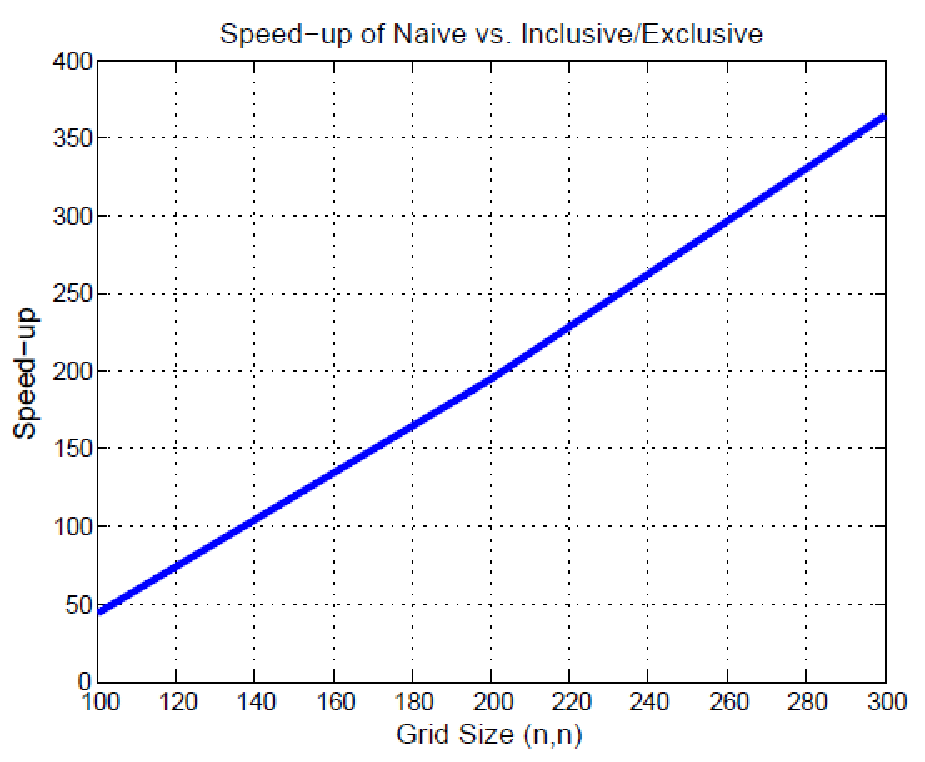
\includegraphics[width=0.4\linewidth]{figtkde/naivespeedup}
\label{fast:subfig1}
}
~~\subfloat[(b) number of rectangles per second processed]{
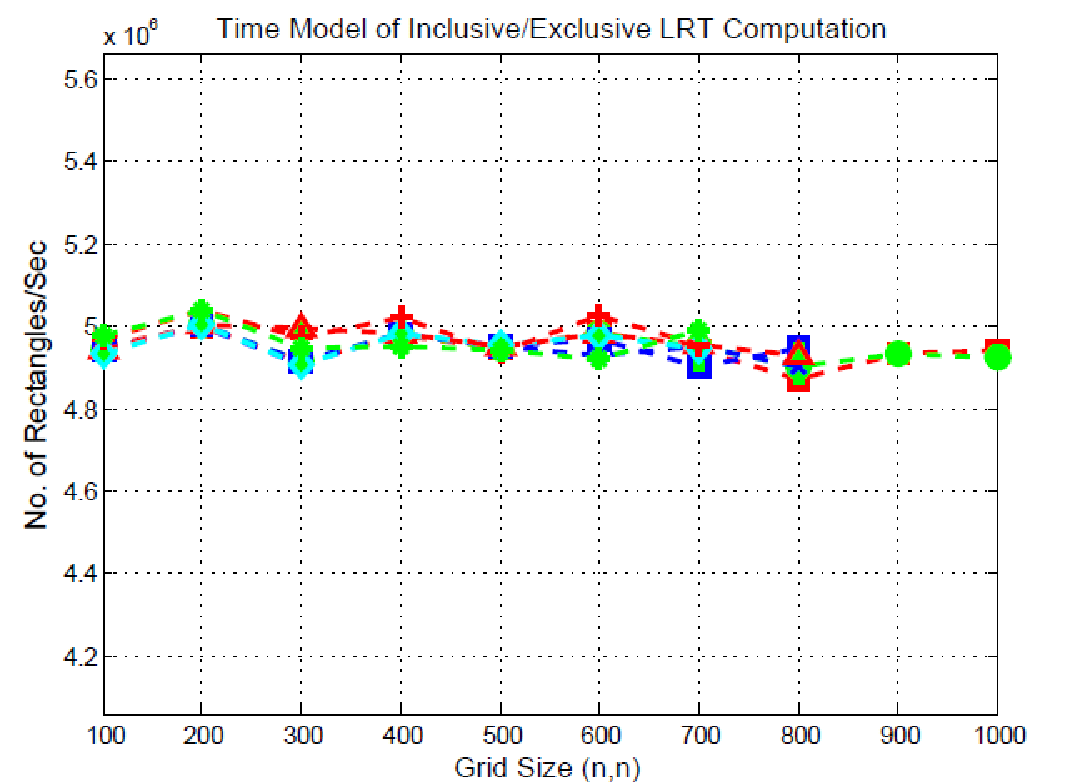
\includegraphics[width=0.45\linewidth]{figtkde/fastspeed}
\label{fast:subfig2}
}
\caption{Naive vs. Inclusive/Exclusive Approach }\label{fast}
\end{figure}

\subsubsection{Multi-core}
 The multi-core experiment is conducted on a 32-core AMD Opteron(tm) Processor 6128 server with 128GB of RAM and a 64-core AMD Opteron(tm) Processor 6378 server with 384GB of RAM. We use data grid with size of (1000,1000) to show the performance scaling. Figure~\ref{multicore:multicore1} and ~\ref{multicore:speedup2} show that the 1EXP-LRT computation scales very well on multi-core architecture.  The speedup increases near-linearly with the increase of number of cores $(no_c)$ and is consistent with the $\bigo(n^4/no_c)$ running time on each core. A speedup of $n$ on $n$ cores is nearly achieved, indicating near perfect scaling.\\
The number of rectangles processed per second is plotted against the number of cores in Figure~\ref{multicore:norectangles} and ~\ref{multicore:norectangles2}. The results show the linearity of increasing number of rectangles processed per second with increasing number of cores.
%multi-core
\begin{figure}[h]
\centering
\subfloat[(a) Speed-up and Efficiency of Grid (1000,1000) on Multi-core]{
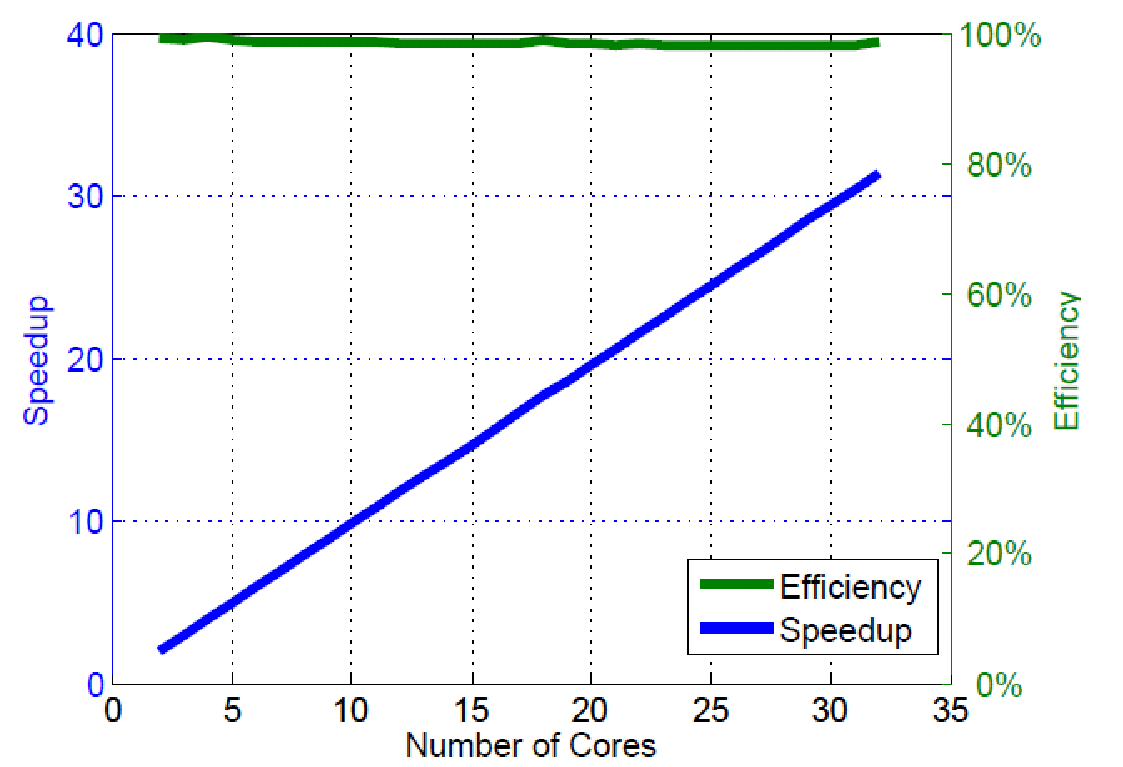
\includegraphics[width=0.48\linewidth]{figtkde/speedup-efficiency}
\label{multicore:multicore1}
}
~~\subfloat[(b) The number of rectangles processed per second vs. number of cores on Grid (1000,1000)]{
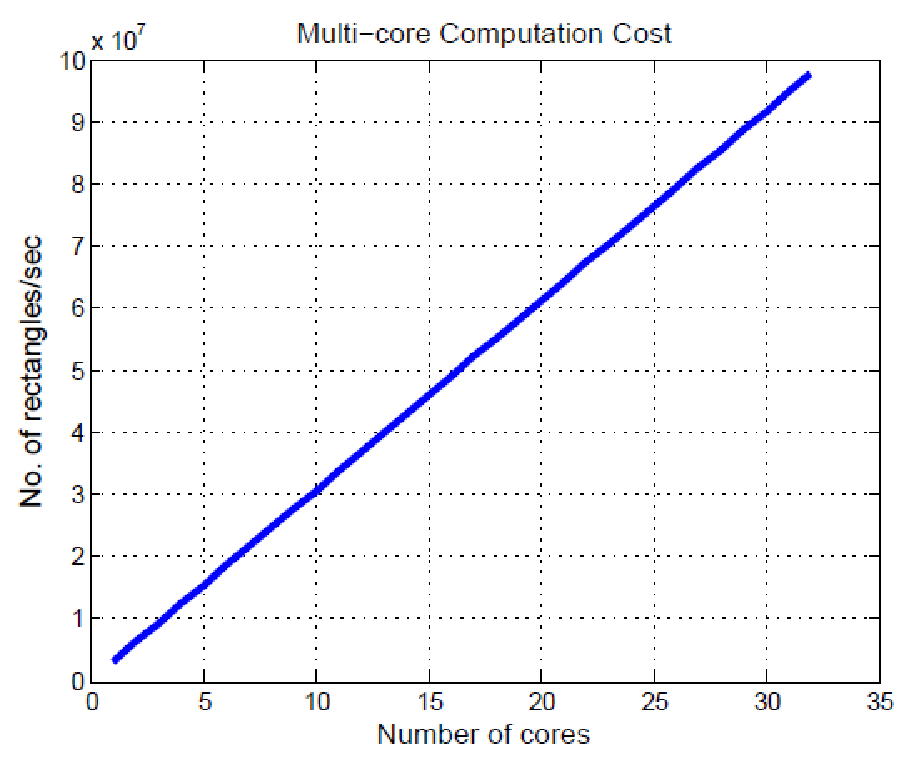
\includegraphics[width=0.41\linewidth]{figtkde/singlerectangle}
\label{multicore:norectangles}
}\\
~~\subfloat[(c) Speed-up and Efficiency of Grid (1000,1000) on Multi-core 2]{
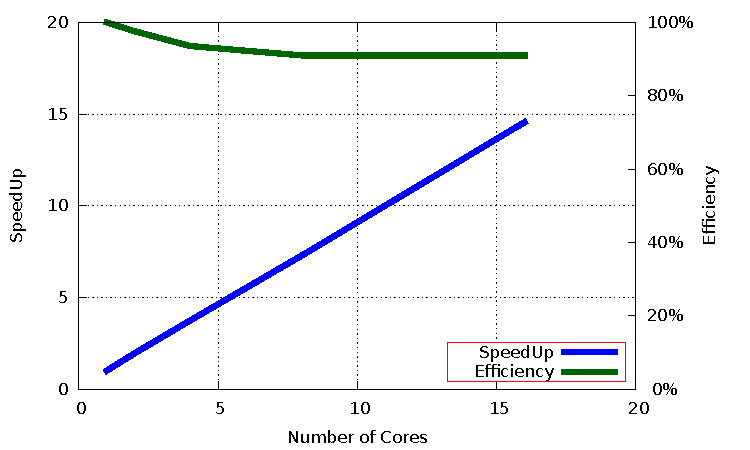
\includegraphics[width=0.49\linewidth]{figtkde/multicore}
\label{multicore:speedup2}
}
~~\subfloat[(d) The number of rectangles processed per second vs. number of cores on Grid (1000,1000) on Multi-core2]{
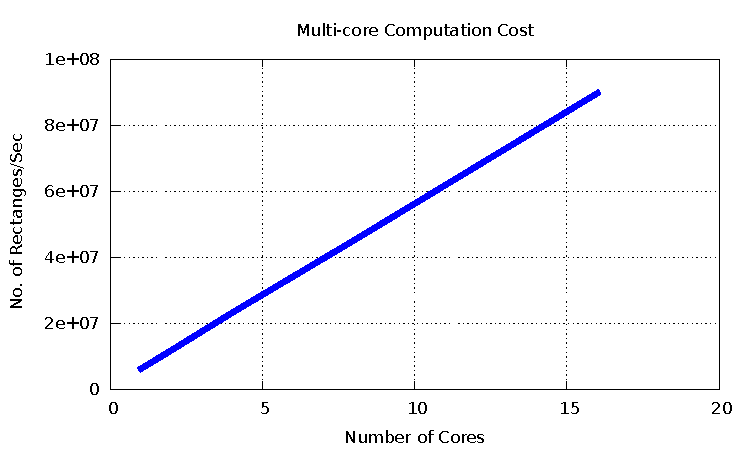
\includegraphics[width=240pt, height=170pt]{figtkde/norec_multicore}
\label{multicore:norectangles2}
}
\caption{Multi-core Evaluation}\label{multicore}
\end{figure}


\subsubsection{Multi-GPGPU}
\noindent The experiments are conducted on two different GPGPU configurations:
\\ (1)An 8-core E5520 Intel server that is equipped with two GPGPU $Tesla$ $C1060$ cards supporting CUDA 4.0. Each GPGPU card has $4GB$ global memory, $16KB$ shared memory, $240$
cores and $30$ multiprocessors. Experiments are conducted to compare the speed-up performance of GPGPUs with exclusive/inclusive cpu approach (see figure~\ref{gpu:subfig1}) on various data grid size (n,n). Furthermore, the performance of number of rectangles processed per second on one single GPGPU vs. two GPGPUs are compared (see figure ~\ref{gpu:subfig2}). The results show that LRT computation on two GPGPUs is around 2 times faster than that on one single GPGPU regardless of the data grid size. And the computation cost of per rectangle is almost constant with the increase of data grid for single GPGPU and two GPGPUs with exclusive/inclusive cpu approach.
\\ (2) An 8-core server that is equipped with two GPGPU $Tesla$ $K20m$ cards supporting CUDA 6.5. Each GPGPU card has $5GB$ global memory,$64KB$ shared memory,$2496$ cores and $13$ multiprocessors. In this architecture, we investigate the speed-up, efficiency and the number of rectangles processed per second with different number of threads on different grid size(see figure ~\ref{gpu:subfig3} and figure ~\ref{gpu:subfig4}). Figure ~\ref{gpu:subfig3} shows the linearly increasing speed-up with increasing number of threads on a given grid size. The efficiency is almost $100\%$. Figure ~\ref{gpu:subfig4} shows the linear increasing speed of processing number of rectangles with the increasing of threads on a given grid size.   \\

%gpu
\begin{figure}[h]
\centering
\subfloat[(a) GPGPU speed-up with inclusive/exclusive cpu approach ]{
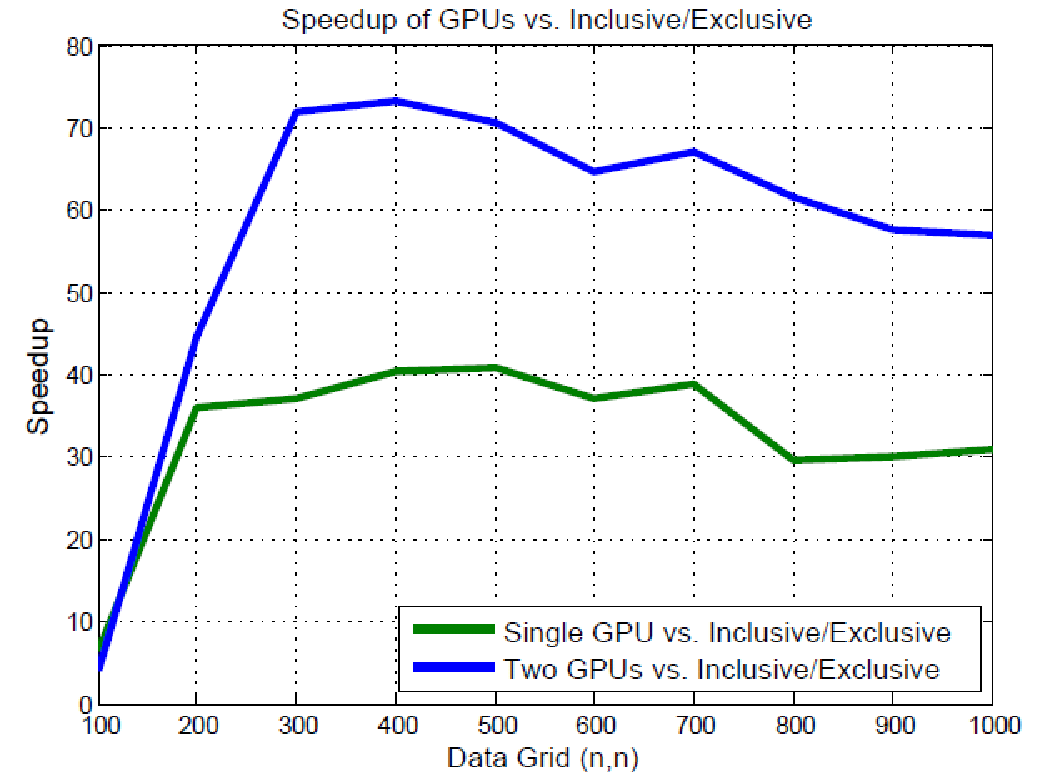
\includegraphics[width=0.45\linewidth]{figtkde/GPUspeedup}
\label{gpu:subfig1}
}
~~\subfloat[(b) Number of rectangles processed per second on single GPGPU vs. two GPGPUs.]{
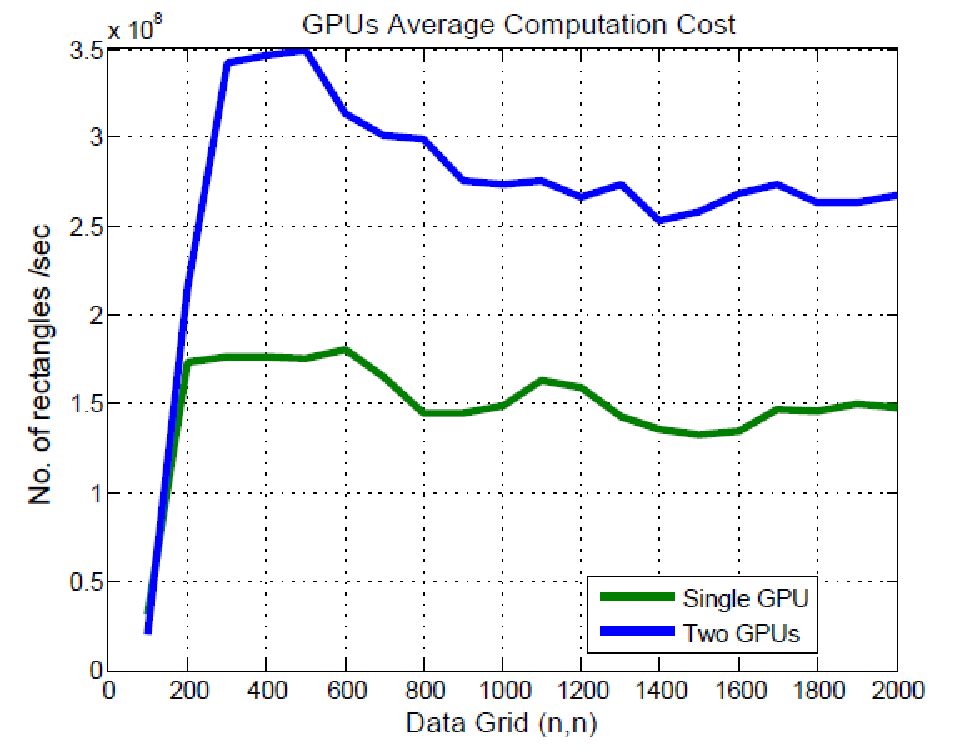
\includegraphics[width=0.45\linewidth]{figtkde/gpurecpersec}
\label{gpu:subfig2}
}\\
~~\subfloat[(c) Speed-up and Efficiency of threads processing on different given grids in GPGPU architecture]{
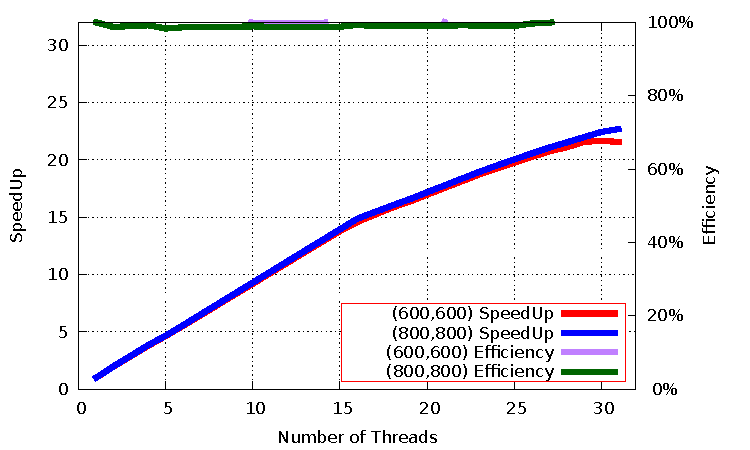
\includegraphics[width=0.5\linewidth]{figtkde/gpuspeff}
\label{gpu:subfig3}
}
~~\subfloat[(d) The number of rectangles processed per second vs. number of threads on different given grids]{
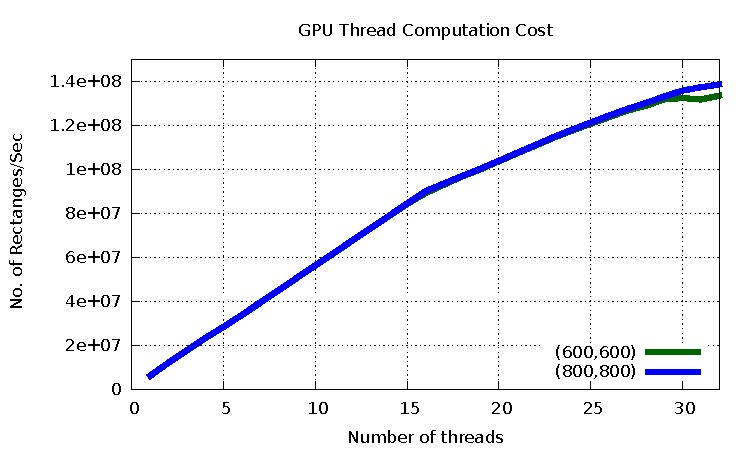
\includegraphics[width=0.5\linewidth]{figtkde/norec_gpu}
\label{gpu:subfig4}
}
\caption{GPGPUs Cost}\label{gpgpus}
\end{figure}



\begin{comment}
\begin{figure}[h]
\centering
\subfloat[]{
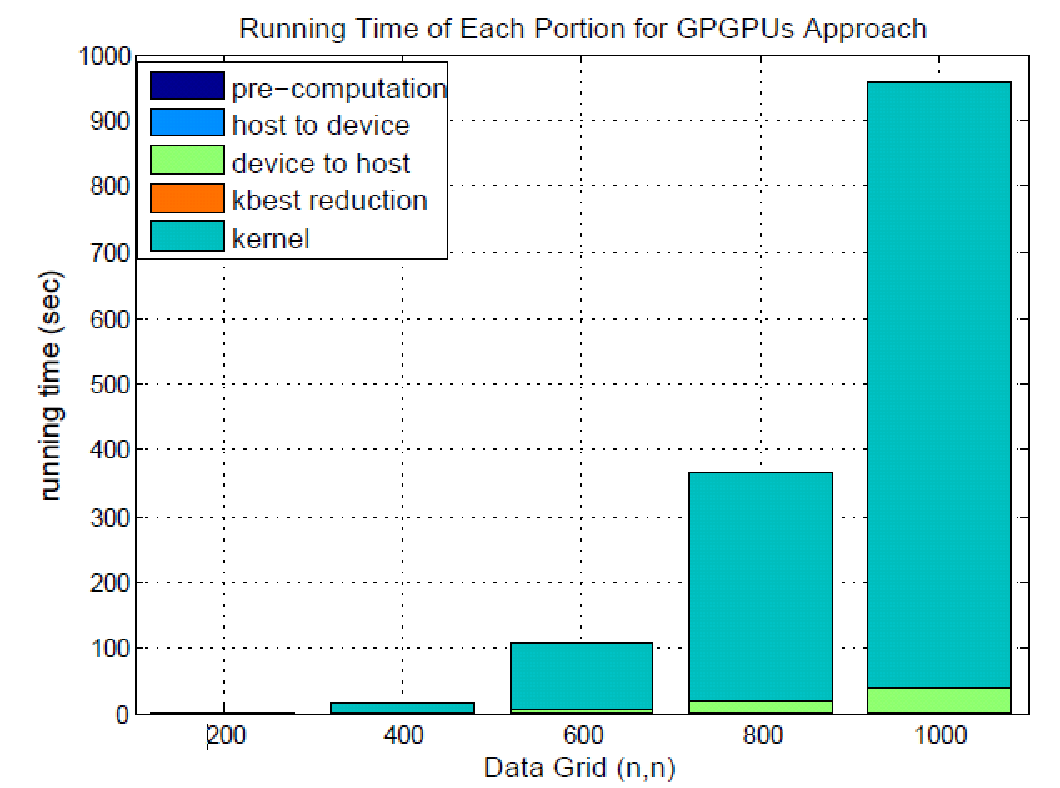
\includegraphics[width=0.9\linewidth]{figtkde/gpuportion}
\label{breakdown:subfig1}
}
\caption{GPGPUs Breakdown parts}\label{breakdown}
\end{figure}
\end{comment}
Given the $((((n+1)\times(n+1))/2)^2)$ regions to be searched for a $(n,n)$ grid and the number of threads in each block is $(tx,ty)$. The number of blocks $(bx,by)$ changes the LRT computation performance. In our implementation,each region object takes $8byte$. To fully utilize the shared memory, each block has $(tx,ty)=(16,8)$ threads. We vary the value of $(bx,by)$ for the grids with different size to find the optimal block configuration. To maximize performance:
\begin{itemize}
\item $Max(blocks)\le (bx\times by)\le ((n+1)\times(n+1)/2)^2$, otherwise some blocks won't work.
\item $((n+1)\times(n+1)/2)^2/(bx\times by)\ge (tx\times ty)$ makes each thread processes at least one region.
\item $((n+1)\times(n+1)/2)^2/tx \le (((n+1)\times(n+1))/2))/ty$ is better for reducing bank conflicts since it retrieves more data by rows.
\end{itemize}
If there are too few blocks, each thread processes a quite number of regions and thus performance is degraded. Table~\ref{tab:op} gives the optimal block configuration. A speedup of up to two can be achieved by choosing the right block configuration using the slowest run for a given grid size as baseline.

\begin{table}[t]
\centering \caption{Optimized Block Configuration\label{tab:op}}
 \begin{tabular}{|c|c|c|}
	\hline
$Grid$ &$block_x$ &$block_y$\\
	\hline
(500,500)     & 128 & 64\\
	\hline
(600,600)     & 192 & 86\\
	\hline
(700,700)     & 176& 86\\
\hline
\end{tabular}
\label{tab:op}
\end{table}

\subsubsection{EC2 Cloud Cluster}
We study a cluster composed of $20 EC2$ high-CPU compute nodes and its effect on MPI application scaling. Instances of this family have proportionally more CPU resources than memory (RAM) and are well suited for compute-intensive applications. Figure~\ref{ec2:subfig1} shows the nearly linear speedup with the increase of number of processes for different grid size on cloud cluster. The computation speed of rectangles is plotted out in Figure~\ref{ec2:subfig2}, it shows the computation speed is faster with the increase number of processes on a given data grid and also verifies the constant computation speed for different data grid by a given number of processes.




%ec2speedup
\begin{figure}[h]
\centering
\subfloat[]{
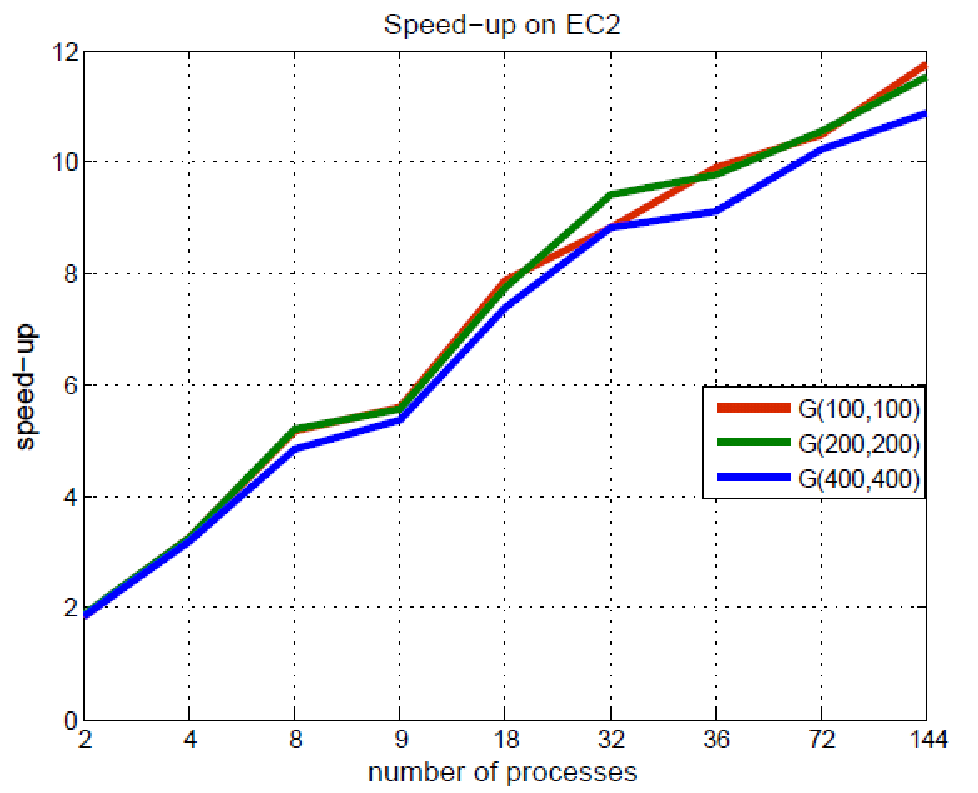
\includegraphics[width=0.45\linewidth]{figtkde/ec2speedup}
\label{ec2:subfig1}
}
~~\subfloat[]{
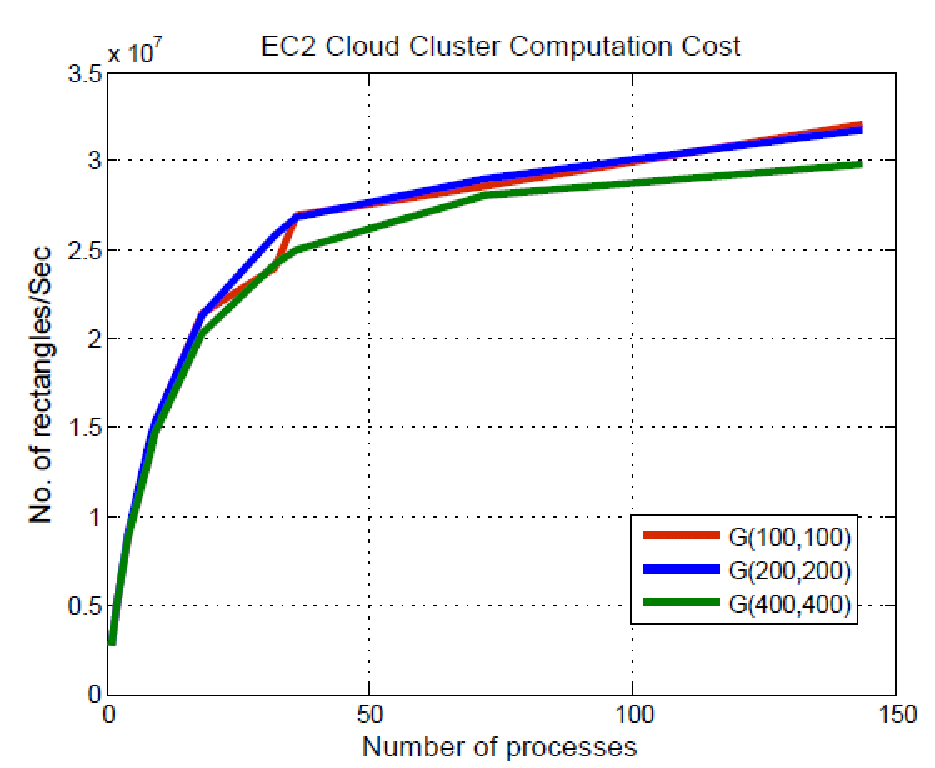
\includegraphics[width=0.45\linewidth]{figtkde/ec2compcost}
\label{ec2:subfig2}
}
\caption{Speed-up of LRT computation on EC2 cloud cluster }\label{ec2}
\end{figure}

\subsection{Discussion}
From the above results, we further analyze of LRT computation on different architectures. We plot the number of rectangles processed per second for data grid $(1000,1000)$ on the following different architectures: multi-core, GPGPU and EC2 cloud cluster. The results are shown in Figure~\ref{cm}. The dashed line in the figure is the processing speed of Inclusive/Exclusive approach on single CPU. From the figure, we can see that the GPGPU approach performs much better than multi-core and EC2, which is almost one order of magnitude faster. Furthermore, we can see that, as the number of cores and the number of processes increase, the LRT processing speed is improved on these architectures. \\

\begin{comment}
\begin{table*}[t]
\begin{tabular}{|l|l|l|l|} \hline
\multicolumn{4}{|c|}{Different Parallel Architectures} \\
\hline
\multirow{1}{*}{}   & Multi-core & GPGPUs & EC2 Cluster  \\
 \hline
\multirow{1}{*}{Factors}   & $(n,nc)$  & $(n,ng,nb)$  & $(n,np)$ \\
 \hline
\multirow{2}{*}{SpeedUp} & (1) linear to $nc$ for a given $n$& (1) almost linear to $ng$ for given $n$ and $nb$ &  (1)linear to $np$ for a given $n$ \\
{} & {}& (2) constant to different $n$ for given ng and nb& {} \\
{} & {}& (3) $\times$(1.5~2.5) by choosing an optimal nb for given $n$ and $ng$ &{}\\
 \hline
 \multirow{2}{*}{$no_r$/sec} & (1) linear to $nc$ for a given $n$&(1)almost constant for a given $n$& \\
 \multirow{2}{*}{} & {}&(2)almost linear to $ng$ for a given $n$& (1)is proportional to $\log (np)$\\
 \hline
\end{tabular}
 \caption{The comparison of different parallel implementations to Inclusive/Exclusive sequential implementation. Note: $n$ is grid size, $nc$ is the number of cores, $ng$ is the number of GPGPUs, $nb$ is the block number for GPGPU kernel and $np$ is the number of processes. }\label{cmtable}
\end{table*}


\begin{figure}[h]
\centering
\subfloat[]{
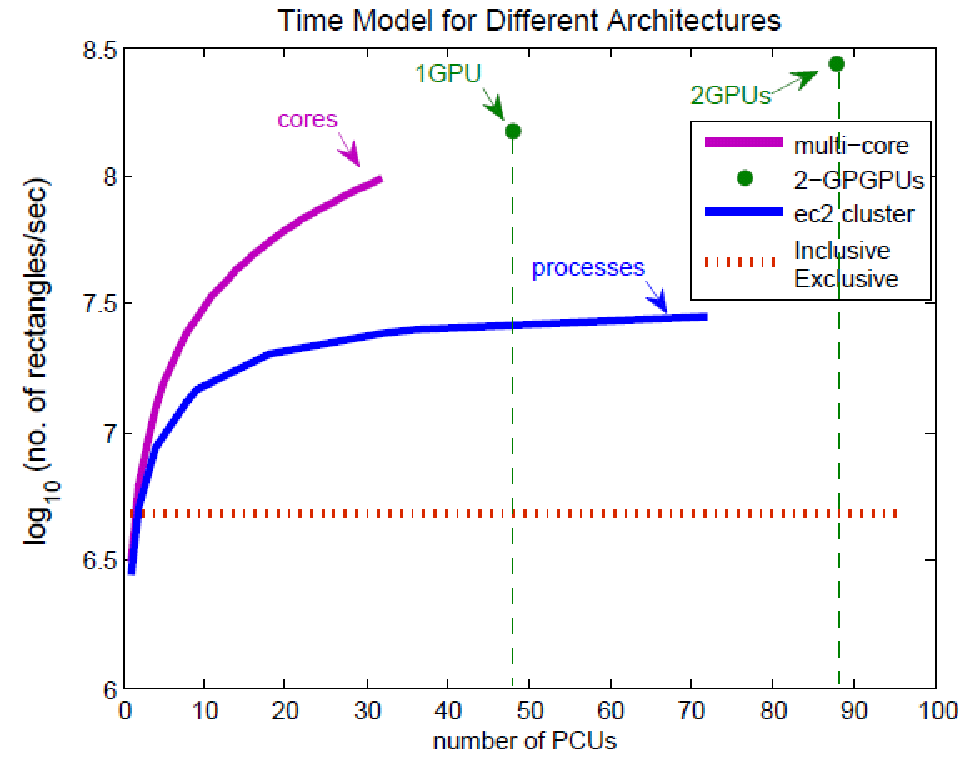
\includegraphics[width=0.85\linewidth]{figtkde/combined}
\label{cm}
}
\caption{Time Model of Different Architectures}\label{cm}
\end{figure}
\end{comment}
\section {Related Work} \label{RW}
Previous attempts to parallelize LRT computation have only achieved limited success. For example, the Spatial Scan Statistic (SSS), which
is a special case of LRT for Poisson data, is available
as a program under the name SatScan~\cite{sat}. It has been parallelized for multi-core CPU environments and its extension for a GPGPU hardware~\cite{Larew} has
achieved improved speed up of two over the multi-core
baseline. The GPGPU implementation in~\cite{Larew} has proposed loading parts
of the data into shared memory but has achieved only a modest speed up. The
other attempt of~\cite{zhao} applied their own implementation of a spatial
scan statistic program on the GPU to the epidemic disease dataset. This solution is only applicable to its special disease scenario.
In each of these cases, we believe there is further room for optimising the
algorithms for the parallel architectures by devising the fine-grained parallelism strategies. Furthermore, these existing parallel solutions perform
LRT tests in a circular or cylindrical way, not in a grid-based scenario. Our parallel
solution is different and provides a fully paralleled template for
1EXP-LRT computation in a grid.

Recently there are some work ~\cite{Power,Neil16,xzhou16,Matheny16} using LRT Framework  to solve the big computation cost, however, they focus on improving pruning strategy, choosing subset or using sampling strategy , not utilizing parallel and distributed architecture to to speed up performance.

\section{Conclusion}\label{CC}
The Likelihood Ratio Test Statistic (LRT) is a state-of-the-art method for identifying hotspots or anomalous
regions in large spatial settings. To speed up the LRT computation for 1EXP family, this paper proposed three ideas: (i) a novel range mapping scheme is proposed to fully enumerate all the regions in a contiguous space. (ii) a dynamic pre-computation algorithm is implemented to reduce the cost of aggregating intermediate statistics. (iii) to save space and improve processing speed, kbest reduction scheme is presented to accumulate distributed results. We did the implementations on different parallel architectures: Multi-core, Multi-GPGPU and EC2 cloud cluster and extensive experiments are done correspondingly. From the results, we see that pre-computation approach has a linear speed-up with the data grid size comparing to the brute-force sequential approach. Then we compare the speed-up on different parallel architectures using pre-computation approach as baseline. The speed-up of these parallel approach increases near-linearly with the increase of the number of ``parallel
computing component'' on different architectures. In concert, the parallel approaches yield a speed up of nearly four thousand times compared to
their sequential counterpart. Further analysis on the processing speed of number of rectangles is given. This provides some recommended information for choosing the right architectures on various factors. Moving the computation of the LRT statistics to the parallel architectures enables the use of this sophisticated method of outlier detection for larger
spatial grids than previously reported.

In future, we will apply the range mapping scheme on non-1EXP family distribution using pruning strategy~\cite{jour}. A unified parallel approach will be provided for generalized LRT computation in spatial grids.

\section*{Supporting information}

\section{Inclusive/Exclusive Statistics Aggregation }

\begin{eqnarray}
|R(x_1,y_1,x_2,y_2)|&= & |A(x_2,y_2)| + |B(x_1,y_1)| + |X(x_1,y_2)| +|Y(x_2,y_1)| - |G|
\end{eqnarray}

\begin{proof}
\begin{eqnarray}
|R|&=\sum_{i=1}^{x_2}\sum_{j=1}^{y_2}c_{i,j}+\sum_{i={x_1}}^{n}\sum_{j={y_1}}^{n}c_{i,j}+\sum_{i={x_2}}^{n}\sum_{j=1}^{y_1}c_{i,j}+\sum_{i=1}^{x_1}\sum_{j={y_2}}^{n}c_{i,j}\\& \quad-\sum_{i=1}^{n}\sum_{j=1}^{n}c_{i,j}\\&\quad=\sum_{i=1}^{x_1}\sum_{j=1}^{y_2}c_{i,j}+\sum_{i={x_1}}^{x_2}(\sum_{j=1}^{y_1}c_{i,j}+\sum_{j={y_1}}^{y_2}c_{i,j})+\sum_{i={x_1}}^{n}\sum_{j={y_1}}^{n}c_{i,j}\\& \quad +\sum_{i={x_2}}^{n}\sum_{j=1}^{y_1}c_{i,j}+\sum_{i=1}^{x_1}\sum_{j={y_2}}^{n}c_{i,j}\\&\quad=\sum_{i=1}^{x_1}\sum_{j=1}^{n}c_{i,j}+\sum_{i={x_1}}^{x_2}\sum_{j=1}^{y_1}c_{i,j}+|R|+|R|+\sum_{i={x_1}}^{x_2}\sum_{j={y_2}}^{n}c_{i,j}\\&\quad+\sum_{i={x_2}}^n\sum_{j=1}^{n}c_{i,j}-\sum_{i=1}^n\sum_{j=1}^{n}c_{i,j}
\\&\quad =\sum_{i=1}^n\sum_{j=1}^{n}c_{i,j}+|R|-\sum_{i=1}^n\sum_{j=1}^{n}c_{i,j}\\&\quad =|R|
\end{eqnarray}
\end{proof}

\begin{definition}
\begin{eqnarray}
A(i,j)=\sum_{k=1}^{i}\sum_{l=1}^{j}c_{i,j}\mbox{\quad for all $1\leq i,j\leq n$}.
\end{eqnarray}
\end{definition}

\begin{lemma}
\begin{eqnarray}
A(i,j)=A_{i-1,j}+A_{i,j-1}-A_{i-1,j-1}+c_{i,j} \mbox{\quad for all $1<i,j\leq n$}.
\end{eqnarray}
\end{lemma}

\begin{proof}
\begin{eqnarray}
A(i,j)& = & \sum_{k=1}^{i-1}\sum_{l=1}^{j}c_{k,l}+a_{i,j-1}-a_{i-1,j-1}+c_{i,j}\\
 & = & \sum_{k=1}^{i-1}\left(\sum_{l=1}^{j-1}c_{k,l}+c_{k,j}\right)+a_{i,j-1}-\sum_{k=1}^{i-1}\sum_{l=1}^{j-1}c_{k,l}+c_{i,j}\\
 & = & \sum_{k=1}^{i-1}c_{k,j}+c_{i,j}+a_{i,j-1}\\
 & = & \sum_{k=1}^{i}c_{k,j}+a_{i,j-1}\\
 & = & \sum_{k=1}^{i}c_{k,j}+\sum_{k=1}^{i}\sum_{l=1}^{j-1}c_{k,l}\\
 & = & A(i,j)
\end{eqnarray}

\end{proof}

\begin{definition}
\begin{equation}
X_{i,j}=\sum_{k=i}^{n}\sum_{l=1}^{j}c_{i,j}\mbox{\quad for all $1\leq i,j\leq n$}.
\end{equation}
\end{definition}

\begin{lemma}
\begin{equation}
X_{i,j}=X_{i,j-1}+X_{i+1,j}-X_{i+1,j-1}+c_{i,j} \mbox{\quad for all $1<i,j\leq n$}.
\end{equation}
\end{lemma}

\begin{proof}
\begin{eqnarray*}
X_{i,j}& = & \sum_{k=i+1}^{n}\sum_{l=1}^{j}c_{k,l}+X_{i,j-1}-X_{i+1,j-1}+c_{i,j}\\
 & = & \sum_{k=i+1}^{n}\left(\sum_{l=1}^{j-1}c_{k,l}+c_{k,j}\right)+X_{i,j-1}-\sum_{k=1+1}^{n}\sum_{l=1}^{j-1}c_{k,l}+c_{i,j}\\
 & = & \sum_{k=i+1}^{n}c_{k,j}+c_{i,j}+X_{i,j-1}\\
 & = & \sum_{k=i}^{n}c_{k,j}+X_{i,j-1}\\
 & = & \sum_{k=i}^{n}c_{k,j}+\sum_{k=i}^{n}\sum_{l=1}^{j-1}c_{k,l}\\
 & = & X_{i,j}
\end{eqnarray*}
\end{proof}

\begin{definition}
\begin{equation}
X_{i,j}=\sum_{k=i}^{n}\sum_{l=1}^{j}c_{i,j}\mbox{\quad for all $1\leq i,j\leq n$}.
\end{equation}
\end{definition}

\begin{lemma}
\begin{equation}
X_{i,j}=X_{i,j-1}+X_{i+1,j}-X_{i+1,j-1}+c_{i,j} \mbox{\quad for all $1<i,j\leq n$}.
\end{equation}
\end{lemma}

\begin{proof}
\begin{eqnarray*}
X_{i,j}& = & \sum_{k=i+1}^{n}\sum_{l=1}^{j}c_{k,l}+X_{i,j-1}-X_{i+1,j-1}+c_{i,j}\\
 & = & \sum_{k=i+1}^{n}\left(\sum_{l=1}^{j-1}c_{k,l}+c_{k,j}\right)+X_{i,j-1}-\sum_{k=1+1}^{n}\sum_{l=1}^{j-1}c_{k,l}+c_{i,j}\\
 & = & \sum_{k=i+1}^{n}c_{k,j}+c_{i,j}+X_{i,j-1}\\
 & = & \sum_{k=i}^{n}c_{k,j}+X_{i,j-1}\\
 & = & \sum_{k=i}^{n}c_{k,j}+\sum_{k=i}^{n}\sum_{l=1}^{j-1}c_{k,l}\\
 & = & X_{i,j}
\end{eqnarray*}
\end{proof}

\begin{definition}
\begin{equation}
y_{i,j}=\sum_{k=1}^{i}\sum_{l=j}^{n}c_{i,j}\mbox{\quad for all $1\leq i,j\leq n$}.
\end{equation}
\end{definition}

\begin{lemma}
\begin{equation}
Y_{i,j}=Y_{i-1,j}+Y_{i,j+1}-Y_{i-1,j+1}+c_{i,j} \mbox{\quad for all $1<i,j\leq n$}.
\end{equation}
\end{lemma}

\begin{proof}
\begin{eqnarray*}
Y_{i,j}& = & \sum_{k=1}^{i-1}\sum_{l=j}^{n}c_{k,l}+Y_{i,j+1}-Y_{i-1,j+1}+c_{i,j}\\
 & = & \sum_{k=1}^{i-1}\left(\sum_{l=j+1}^{n}c_{k,l}+c_{k,j}\right)+Y_{i,j+1}-\sum_{k=1}^{i-1}\sum_{l=j+1}^{n}c_{k,l}+c_{i,j}\\
 & = & \sum_{k=1}^{i-1}c_{k,j}+c_{i,j}+Y_{i,j+1}\\
 & = & \sum_{k=1}^{i}c_{k,j}+Y_{i,j+1}\\
 & = & \sum_{k=1}^{i}c_{k,j}+\sum_{k=1}^{i}\sum_{l=j+1}^{n}c_{k,l}\\
 & = & Y_{i,j}
\end{eqnarray*}
\end{proof}

\section{Pre-processing of Inclusive/Exclusive Computation}
\begin{algorithm}[t!]
\label{pre1}
\caption{Inclusive/Exclusive Pre-computation for Set B}\label{pre1}
Input: data grid (G) \\
Output: accumulated counts $B(i,j)$\\
------------------------------------------------------------------ \\
\begin{algorithmic}[1]
\State //Initialize first element $B(n-1,n-1)$
\State {\textit { $B(n-1,n-1)$\(\leftarrow\)$G(n-1,n-1)$}}
\State //accumulation of remaining elements in last column
\For{\textit  j\(\leftarrow\)(n-1) to \textit{1}}
\State{\textit { $B(j-1,n-1)$ \(\leftarrow\) $G(i-1,n-1)$ +$B(j,n-1)$}}
\EndFor
\State //accumulation of remaining elements in last row
\For{\textit  i\(\leftarrow\)(n-1) to \textit{1}}
\State  {\textit {$B(n-1,i-1)$\(\leftarrow\)$G(n-1,i-1)$ + $B(n-1,i)$}}
\EndFor
\State //accumulation of all the elements in remaining rows and columns
\For{\textit  k\(\leftarrow\)1 to \textit{n}}
\For{\textit  i\(\leftarrow\)(n-1) to \textit{k}}
\State  {\textit B(i-k,n-1-k)\(\leftarrow\) G(i-k,n-1-k)+B(i-k+1,n-1-k)+B(i-k,n-k)-B(i-k+1,n-k)}
\EndFor
\For{\textit  j\(\leftarrow\)(n-1) to \textit{k}}
\State  {\textit B(n-1-k,j-k)\(\leftarrow\)G(n-1-k,j-k)+B(n-1-k,j-k+1)+ B(n-k,j-k)-B(n-k,j-k+1)}
\EndFor
\EndFor
\end{algorithmic}
\end{algorithm}

\begin{algorithm}[t!]
\label{pre2}
\caption{Pre-processing of Inclusive/Exclusive Computation for Set X}\label{pre2}
------------------------------------------------------------------ \\
\begin{algorithmic}[1]
\State //Initialize first column
\For{\textit  i\(\leftarrow\)1 to \textit{n}}
\State {\textit {X(i,0)\(\leftarrow\)0 }}
\EndFor
\State //Initialize last row
\For{\textit  j\(\leftarrow\)1 to \textit{n}}
\State  {\textit { X(n-1,j)\(\leftarrow\)0 }}
\EndFor
\State //Iterate over all diagonal elements
\For{\textit  k\(\leftarrow\)1 to \textit{n}}
\State //associate columns of diagonal elements
\For{\textit  i\(\leftarrow\)n-1 to \textit k}
\State  {\textit X(i-k,k)\(\leftarrow\)G(i-k+1,k-1)+X(i-k+1,k)+X(i-k,k-1)-X(i-k+1,k-1)}
\EndFor
\State // associate columns of diagonal element k
\For{\textit j\(\leftarrow\)k to \textit{n}}
\State  {\textit X(n-1-k,j)\(\leftarrow\)G(n-k,j-1)+X(n-1-k,j-1)+X(n-k,j)-X(n-k,j-1)}
\EndFor
\EndFor
\end{algorithmic}
\end{algorithm}

\begin{algorithm}[t!]
\label{pre1}
\caption{Inclusive/Exclusive Pre-computation for Set Y}\label{pre1}
Input: data grid (G) \\
Output: accumulated counts $Y(i,j)$\\
------------------------------------------------------------------ \\
\begin{algorithmic}[1]
\State //Initialize last column
\For{\textit  i\(\leftarrow\)1 to \textit{n}}
\State {\textit {Y(i,n-1)\(\leftarrow\)0 }}
\EndFor
\State //Initialize first row
\For{\textit  j\(\leftarrow\)1 to \textit{n}}
\State  {\textit { Y(0,j)\(\leftarrow\)0 }}
\EndFor
\State //Iterate over all diagonal elements
\For{\textit  k\(\leftarrow\)1 to \textit{n}}
\State //associate columns of diagonal elements
\For{\textit  i\(\leftarrow\)k to \textit (n-1)}
\State  {\textit Y(i,n-1-k)\(\leftarrow\)G(i-1,n-k)+Y(i-1,n-1-k)+ Y(i,n-k)-Y(i-1,n-k)}
\EndFor
\State // associate columns of diagonal element k
\For{\textit j\(\leftarrow\)(n-1) to \textit{k}}
\State  {\textit Y(k,n-k)\(\leftarrow\)G(k-1,n-k+1)+Y(k,n-k+1)+Y(k-1,n-k)-Y(k-1,n-k+1)}
\EndFor
\EndFor
\end{algorithmic}
\end{algorithm}

%\nocite{*}% Show all bib entries - both cited and uncited; comment this line to view only cited bib entries;
\bibliography{gpulrt}%wileyNJD-AMA

\clearpage

\end{document}
